% Options for packages loaded elsewhere
\PassOptionsToPackage{unicode}{hyperref}
\PassOptionsToPackage{hyphens}{url}
\PassOptionsToPackage{dvipsnames,svgnames,x11names}{xcolor}
%
\documentclass[
]{article}

\usepackage{amsmath,amssymb}
\usepackage{iftex}
\ifPDFTeX
  \usepackage[T1]{fontenc}
  \usepackage[utf8]{inputenc}
  \usepackage{textcomp} % provide euro and other symbols
\else % if luatex or xetex
  \usepackage{unicode-math}
  \defaultfontfeatures{Scale=MatchLowercase}
  \defaultfontfeatures[\rmfamily]{Ligatures=TeX,Scale=1}
\fi
\usepackage{lmodern}
\ifPDFTeX\else  
    % xetex/luatex font selection
\fi
% Use upquote if available, for straight quotes in verbatim environments
\IfFileExists{upquote.sty}{\usepackage{upquote}}{}
\IfFileExists{microtype.sty}{% use microtype if available
  \usepackage[]{microtype}
  \UseMicrotypeSet[protrusion]{basicmath} % disable protrusion for tt fonts
}{}
\usepackage{xcolor}
\setlength{\emergencystretch}{3em} % prevent overfull lines
\setcounter{secnumdepth}{5}
% Make \paragraph and \subparagraph free-standing
\ifx\paragraph\undefined\else
  \let\oldparagraph\paragraph
  \renewcommand{\paragraph}[1]{\oldparagraph{#1}\mbox{}}
\fi
\ifx\subparagraph\undefined\else
  \let\oldsubparagraph\subparagraph
  \renewcommand{\subparagraph}[1]{\oldsubparagraph{#1}\mbox{}}
\fi

\usepackage{color}
\usepackage{fancyvrb}
\newcommand{\VerbBar}{|}
\newcommand{\VERB}{\Verb[commandchars=\\\{\}]}
\DefineVerbatimEnvironment{Highlighting}{Verbatim}{commandchars=\\\{\}}
% Add ',fontsize=\small' for more characters per line
\usepackage{framed}
\definecolor{shadecolor}{RGB}{241,243,245}
\newenvironment{Shaded}{\begin{snugshade}}{\end{snugshade}}
\newcommand{\AlertTok}[1]{\textcolor[rgb]{0.68,0.00,0.00}{#1}}
\newcommand{\AnnotationTok}[1]{\textcolor[rgb]{0.37,0.37,0.37}{#1}}
\newcommand{\AttributeTok}[1]{\textcolor[rgb]{0.40,0.45,0.13}{#1}}
\newcommand{\BaseNTok}[1]{\textcolor[rgb]{0.68,0.00,0.00}{#1}}
\newcommand{\BuiltInTok}[1]{\textcolor[rgb]{0.00,0.23,0.31}{#1}}
\newcommand{\CharTok}[1]{\textcolor[rgb]{0.13,0.47,0.30}{#1}}
\newcommand{\CommentTok}[1]{\textcolor[rgb]{0.37,0.37,0.37}{#1}}
\newcommand{\CommentVarTok}[1]{\textcolor[rgb]{0.37,0.37,0.37}{\textit{#1}}}
\newcommand{\ConstantTok}[1]{\textcolor[rgb]{0.56,0.35,0.01}{#1}}
\newcommand{\ControlFlowTok}[1]{\textcolor[rgb]{0.00,0.23,0.31}{#1}}
\newcommand{\DataTypeTok}[1]{\textcolor[rgb]{0.68,0.00,0.00}{#1}}
\newcommand{\DecValTok}[1]{\textcolor[rgb]{0.68,0.00,0.00}{#1}}
\newcommand{\DocumentationTok}[1]{\textcolor[rgb]{0.37,0.37,0.37}{\textit{#1}}}
\newcommand{\ErrorTok}[1]{\textcolor[rgb]{0.68,0.00,0.00}{#1}}
\newcommand{\ExtensionTok}[1]{\textcolor[rgb]{0.00,0.23,0.31}{#1}}
\newcommand{\FloatTok}[1]{\textcolor[rgb]{0.68,0.00,0.00}{#1}}
\newcommand{\FunctionTok}[1]{\textcolor[rgb]{0.28,0.35,0.67}{#1}}
\newcommand{\ImportTok}[1]{\textcolor[rgb]{0.00,0.46,0.62}{#1}}
\newcommand{\InformationTok}[1]{\textcolor[rgb]{0.37,0.37,0.37}{#1}}
\newcommand{\KeywordTok}[1]{\textcolor[rgb]{0.00,0.23,0.31}{#1}}
\newcommand{\NormalTok}[1]{\textcolor[rgb]{0.00,0.23,0.31}{#1}}
\newcommand{\OperatorTok}[1]{\textcolor[rgb]{0.37,0.37,0.37}{#1}}
\newcommand{\OtherTok}[1]{\textcolor[rgb]{0.00,0.23,0.31}{#1}}
\newcommand{\PreprocessorTok}[1]{\textcolor[rgb]{0.68,0.00,0.00}{#1}}
\newcommand{\RegionMarkerTok}[1]{\textcolor[rgb]{0.00,0.23,0.31}{#1}}
\newcommand{\SpecialCharTok}[1]{\textcolor[rgb]{0.37,0.37,0.37}{#1}}
\newcommand{\SpecialStringTok}[1]{\textcolor[rgb]{0.13,0.47,0.30}{#1}}
\newcommand{\StringTok}[1]{\textcolor[rgb]{0.13,0.47,0.30}{#1}}
\newcommand{\VariableTok}[1]{\textcolor[rgb]{0.07,0.07,0.07}{#1}}
\newcommand{\VerbatimStringTok}[1]{\textcolor[rgb]{0.13,0.47,0.30}{#1}}
\newcommand{\WarningTok}[1]{\textcolor[rgb]{0.37,0.37,0.37}{\textit{#1}}}

\providecommand{\tightlist}{%
  \setlength{\itemsep}{0pt}\setlength{\parskip}{0pt}}\usepackage{longtable,booktabs,array}
\usepackage{calc} % for calculating minipage widths
% Correct order of tables after \paragraph or \subparagraph
\usepackage{etoolbox}
\makeatletter
\patchcmd\longtable{\par}{\if@noskipsec\mbox{}\fi\par}{}{}
\makeatother
% Allow footnotes in longtable head/foot
\IfFileExists{footnotehyper.sty}{\usepackage{footnotehyper}}{\usepackage{footnote}}
\makesavenoteenv{longtable}
\usepackage{graphicx}
\makeatletter
\def\maxwidth{\ifdim\Gin@nat@width>\linewidth\linewidth\else\Gin@nat@width\fi}
\def\maxheight{\ifdim\Gin@nat@height>\textheight\textheight\else\Gin@nat@height\fi}
\makeatother
% Scale images if necessary, so that they will not overflow the page
% margins by default, and it is still possible to overwrite the defaults
% using explicit options in \includegraphics[width, height, ...]{}
\setkeys{Gin}{width=\maxwidth,height=\maxheight,keepaspectratio}
% Set default figure placement to htbp
\makeatletter
\def\fps@figure{htbp}
\makeatother

\usepackage{booktabs}
\usepackage{longtable}
\usepackage{array}
\usepackage{multirow}
\usepackage{wrapfig}
\usepackage{float}
\usepackage{colortbl}
\usepackage{pdflscape}
\usepackage{tabu}
\usepackage{threeparttable}
\usepackage{threeparttablex}
\usepackage[normalem]{ulem}
\usepackage{makecell}
\usepackage{xcolor}
\usepackage[noblocks]{authblk}
\renewcommand*{\Authsep}{, }
\renewcommand*{\Authand}{, }
\renewcommand*{\Authands}{, }
\renewcommand\Affilfont{\small}
\usepackage{mathtools}
\usepackage[sort, round]{natbib}
\usepackage[left]{lineno}
\usepackage{tabularx}
\linenumbers
\usepackage[a4paper, total={6in, 10in}]{geometry}
\usepackage{longtable}
\usepackage[colorlinks=true,linkcolor=black,citecolor=black,urlcolor=black]{hyperref}
\usepackage{amsmath,amssymb,amsfonts,amsthm}
\usepackage{multirow}
\usepackage{setspace}\doublespacing
\renewcommand{\abstractname}{Summary}
\usepackage{bm}
\usepackage{algorithm}
\usepackage{algpseudocode}
\usepackage{rotating}
\makeatletter
\makeatother
\makeatletter
\makeatother
\makeatletter
\@ifpackageloaded{caption}{}{\usepackage{caption}}
\AtBeginDocument{%
\ifdefined\contentsname
  \renewcommand*\contentsname{Table of contents}
\else
  \newcommand\contentsname{Table of contents}
\fi
\ifdefined\listfigurename
  \renewcommand*\listfigurename{List of Figures}
\else
  \newcommand\listfigurename{List of Figures}
\fi
\ifdefined\listtablename
  \renewcommand*\listtablename{List of Tables}
\else
  \newcommand\listtablename{List of Tables}
\fi
\ifdefined\figurename
  \renewcommand*\figurename{Figure}
\else
  \newcommand\figurename{Figure}
\fi
\ifdefined\tablename
  \renewcommand*\tablename{Table}
\else
  \newcommand\tablename{Table}
\fi
}
\@ifpackageloaded{float}{}{\usepackage{float}}
\floatstyle{ruled}
\@ifundefined{c@chapter}{\newfloat{codelisting}{h}{lop}}{\newfloat{codelisting}{h}{lop}[chapter]}
\floatname{codelisting}{Listing}
\newcommand*\listoflistings{\listof{codelisting}{List of Listings}}
\makeatother
\makeatletter
\@ifpackageloaded{caption}{}{\usepackage{caption}}
\@ifpackageloaded{subcaption}{}{\usepackage{subcaption}}
\makeatother
\makeatletter
\@ifpackageloaded{tcolorbox}{}{\usepackage[skins,breakable]{tcolorbox}}
\makeatother
\makeatletter
\@ifundefined{shadecolor}{\definecolor{shadecolor}{rgb}{.97, .97, .97}}
\makeatother
\makeatletter
\makeatother
\makeatletter
\makeatother
\ifLuaTeX
  \usepackage{selnolig}  % disable illegal ligatures
\fi
\usepackage[]{natbib}
\bibliographystyle{plainnat}
\IfFileExists{bookmark.sty}{\usepackage{bookmark}}{\usepackage{hyperref}}
\IfFileExists{xurl.sty}{\usepackage{xurl}}{} % add URL line breaks if available
\urlstyle{same} % disable monospaced font for URLs
\hypersetup{
  pdftitle={Using NIMBLE to implement Markov Chain Monte Carlo with Integrated Nested Laplace approximation},
  pdfauthor={Kwaku Peprah Adjei; Robert B. O'Hara},
  colorlinks=true,
  linkcolor={black},
  filecolor={Maroon},
  citecolor={black},
  urlcolor={Blue},
  pdfcreator={LaTeX via pandoc}}

\title{Using NIMBLE to implement Markov Chain Monte Carlo with
Integrated Nested Laplace approximation}


\author[1,2]{Kwaku Peprah Adjei}
\author[1,2]{Robert B. O'Hara}

\affil[1]{Department of Mathematical Sciences, Norwegian University of
Science and Technology, Trondheim Norway}
\affil[2]{Center for Biodiversity Dynamics, Norwegian University of
Science and Technology, Trondheim Norway}


\date{}
\begin{document}
\maketitle
\begin{abstract}
\noindent 1. Bayesian inference using Markov Chain Monte Carlo (MCMC)
and Integrated Nested Laplace approximation (INLA) are popular in
applied statistics. MCMC can be slow to run for some models and INLA is
also limited in the class of models it can fit. However, it is possible
to combine INLA with MCMC to fit the class of models that INLA cannot
fit. The MCMC with INLA approach involves dividing the set of parameters
we aim at estimating into two: one that needs to sampled from MCMC
before INLA can be used to fit a model given the sampled parameters.
\newline 2. In this study, we propose that NIMBLE be used to implement
the MCMC with INLA methodology. We do this by proposing two approaches:
a) using INLA-defined functions to write customized samplers in NIMBLE
and b) writing a NIMBLE distribution function with the embedded INLA
function. The approaches are applied to various class of models.
\newline 3. The posterior marginals of the model parameters from the
MCMC with INLA using NIMBLE approaches were consistently similar to
those from MCMC and/or INLA only. \newline \textbf{keywords}: Bayesian
inference, Metropolis-Hastings algorithm, spatial occupancy model,
binomial N-Mixture model
\end{abstract}
\ifdefined\Shaded\renewenvironment{Shaded}{\begin{tcolorbox}[breakable, enhanced, sharp corners, borderline west={3pt}{0pt}{shadecolor}, frame hidden, interior hidden, boxrule=0pt]}{\end{tcolorbox}}\fi

\hypertarget{introduction}{%
\section{Introduction}\label{introduction}}

Bayesian inference has gained popularity in applied statistics, with its
applications spanning the breadth of multiple disciplines. Their
popularity can be attributed to the flexibility it provides
statisticians in fitting models \citep{blangiardo2015spatial}. Markov
chain Monte Carlo (MCMC) method is one of the common approaches used for
Bayesian inference
\citep{gilks1995markov, brooks2011handbook, blangiardo2015spatial, kery2015applied},
due to its easy implementation with open software like JAGS
\citep{hornik2003jags}, WinBUGS \citep{spiegelhalter2014winbugs}, Stan
\citep{carpenter2017stan}, NIMBLE \citep{nimblearticle}. MCMC runs
faster for simple models; however, using MCMC to fit complex models such
as spatio-temporal state space models with large datasets can be very
time consuming \citep{blangiardo2015spatial, kery2020applied}.

Alternatively, integrated nested Laplace approximation (INLA) was
proposed by \citet{rue2009approximate} for Bayesian inference on
hierarchical models that can be represented as latent Gaussian models.
INLA provides a deterministic or numerical algorithm that approximates
the marginal distribution of the latent states, which is the objective
of Bayesian inference \citep{blangiardo2015spatial}. Models fitted with
INLA take a fraction of time MCMC methods take
\citep{blangiardo2015spatial,gomez2018markov}, but still provides
accurate estimates of model parameters
\citep{berild2022importance, gomez2018markov}. In addition, INLA is
available in an R-package \textbf{R-INLA} \citep{rue2009approximate},
providing users with the platform to fit complex hierarchical models in
a matter of seconds. These reasons have made INLA a popular method to
fit hierarchical models. Notwithstanding, there is a limitation in the
class of models that can be fitted with \textbf{R-INLA}. For instance,
models with missing covariates and mixture models cannot be fitted with
\textbf{R-INLA}
\citep{gomez2018markov, berild2022importance, marin2005bayesian}.

To widen the scope of models that can be fitted using INLA, attempts
have been made at fitting conditional linear Gaussian models with
\textbf{R-INLA}
\citep{li2012spatial, bivand2014approximate, gomez2018markov, berild2022importance}.
These conditional models are developed by fixing some of the parameters
in the full model. The values of the fixed parameters can be obtained
from their maximum likelihood estimates \citep{li2012spatial} or from
their posterior distribution estimated with either MCMC
\citep{gomez2018markov, bivand2014approximate} or other Monte Carlo
methods like (adaptive) importance sampling
\citep{berild2022importance}. The values of the fixed parameters can be
plugged into the overall model, and the conditional model can then be
fitted with \textbf{R-INLA}.

This study will focus on the approach by \citet{gomez2018markov}, where
the marginal likelihood of the fitted conditional model is computed with
\textbf{R-INLA}, and this marginal likelihood is used to calculate the
acceptance probability in the Metropolis-Hastings algorithm for the MCMC
method. Our study provides further advancement in the development of
this INLA-MCMC methodology by proposing that NIMBLE (a system for
programming statistical algorithms for general model structures within
R; \citet{nimblearticle}) can be used to implement this approach. The
reasons for this proposal are discussed as follows.

Firstly, NIMBLE is designed to provide flexible model specifications by
extending the BUGS language to include R-defined functions
\citep{nimblemanual}. NIMBLE also provides a programming language for
algorithms and a balance between high-level programmability and
execution efficiency by compiling models and functions via C++
\citep{nimblearticle, nimblemanual}. This means that the computational
time of fitting models with the MCMC-INLA method can be considerably
reduced.

In addition, NIMBLE has been implemented as an R-package,
\textbf{nimble} \citep{nimblePackage}, making both NIMBLE and INLA
readily accessible to users on the same platform. As mentioned already,
NIMBLE provides a platform to integrate R-defined functions within its
BUGS framework \citep{nimblemanual}. This means the conditional model
that we intend to fit using \textbf{R-INLA} can be written as a function
in \(R\) \citep{Rsoftware} and integrated within the BUGS code to be run
with \textbf{nimble}. This makes it possible to utilize the several
sampling algorithms implemented in R-package \textbf{nimble} - without
writing a new sampling algorithm - to obtain the posterior distribution
of the fixed parameters, instead of just the Metropolis-Hasting
algorithm used by \cite{gomez2018markov}. The implemented samplers in
\textbf{nimble} include adaptive (block) random walk, slice sampler,
conjugate (``Gibbs'') samplers, binary sampler, cross level sampler,
categorical sampler, elliptical slice sampler, automated factor slice
sampler, Hamiltonian Monte Carlo sampler \citep{nimblemanual}.

New sampling algorithms other than those implemented in \textbf{nimble}
will be needed for the INLA-MCMC methodology in some instances. These
instances include customizing the sampling algorithm to reduce the
number of calls made to \textbf{R-INLA}, either by parallelizing the
method by using importance sampling instead of MCMC
\citep{berild2022importance}, or specifying how many times
\textbf{R-INLA} should be called by a sampler. This is possible with
\textbf{nimble}, since NIMBLE provides a simple platform for users to
easily implement a customized sampler of their choice (the reader is
referred to the NIMBLE manual \citet{nimblemanual} for further details
on how to write customized samplers in NIMBLE).

This study proposes two alternative ways to implement the INLA-MCMC
approach with NIMBLE. The first alternative involves writing an
\textbf{R-INLA} function to return the marginal likelihood and samples
from the latent states posterior distribution obtained from the fitted
conditional model. A customised sampler is then defined to use this
marginal likelihood in the sampler's decision process to generate
samples of the fixed parameters. If the proposed samples of the fixed
parameters are accepted, then the samples from the fitted conditional
models are also saved; if the proposed samples are rejected, the
posterior samples from the fitted conditional models are not saved. We
write a customized random-walk block (RW) to implement this alternative.

The second alternative involves writing an \textbf{R-INLA} function to
fit the conditional model, and then defining a NIMBLE distribution
function that uses this defined \textbf{R-INLA} function. The
distribution function is integrated into the BUGS code that will be used
to fit the model with \textbf{nimble}. This alternative does not require
new samplers to be written in \textbf{nimble}, but it utilizes the
sampling algorithms already implemented in the R-package
\textbf{nimble}.

We apply the two alternative approaches to fit various models with two
simulated datasets and three real datasets. The bivariate regression
model is fitted to the first simulated dataset and spatial occupancy
model is fitted to the second simulated dataset. The proposed approaches
are also used to fit the Bayesian lasso regression model to the
\textit{Hitters} dataset \citep{gareth2013introduction}, impute missing
covariates with the \textit{nhanes} dataset
\citep[accessed from ][]{van2011mice}, zero-inflated Poisson model with
data on the number of fishes caught
\citep[data retrieved from ][]{berild2022importance} and a binomial
N-Mixture model for the mallard dataset
\citep[accessed from R-package \textbf{unmarked}][]{unmarked}. The
results from our proposed approaches are compared to those obtained from
MCMC methods using \textbf{nimble} and maximum likelihood estimation
from some R-packages. This study does not make comparison with the INLA
with Metropolis-Hastings approach by \cite{gomez2018markov}, as we are
only interested in implementing the INLA-MCMC methodology with
\textbf{nimble}. Various summaries of the posterior marginal of the
model parameters are presented, either numerically or graphically.

\hypertarget{integrated-nested-laplace-approxmation}{%
\section{Integrated Nested Laplace
Approxmation}\label{integrated-nested-laplace-approxmation}}

Let \(\mathbf{y} = \{y_1, \ldots, y_n\}\) be observations from an
exponential family, with each observation \(y_i\) for
\(i = 1, 2, \ldots, n\) having mean \(\mu_i\). The mean \(\mu_i\) is
related to some linear predictor (\(\eta_i\)), defined as a combination
of covariates and other functions using an additive structure and an
appropriate link function g(.). The linear predictor can be defined as:
\begin{equation}\label{linpred}
\eta_i = \beta_0 + \sum_{m = 1}^M \beta_m u_{mi} + \sum_{j = 1}^L f_{j}(v_{ji}) + \epsilon_i,
\end{equation} where \(\beta_0\) is the intercept, \(\beta_m\) is the
linear effects of covariate \(u_m\) on the response, \(f_l(.)\) defines
the set of functions of covariate \(v_j\) which can be a smooth or
non-linear effect, trend effect, etc. The unobserved latent effects
\(\eta\), \(\beta_0\), \(\{\beta_m\}_{m=1}^{M}\) are represented by the
vector \(\mathbf{x}\) in this study. Moreover, the conditional
distribution of the latent field and the likelihood are assumed to
depend on some hyperparameters, say \(\mathbb{\theta_1}\) and
\(\mathbb{\theta_2}\) (which could be the residual variance)
respectively. We use \(\mathbb{\theta}\) as an assemblage for both
hyperparameters, i.e,
\(\mathbb{\theta} = (\mathbb{\theta_1}, \mathbb{\theta_2})\).

It is clear from equation \eqref{linpred} that the observations are
conditionally independent given the latent states and the
hyperparameters. Therefore, the likelihood can be written as:

\begin{equation}\label{likelihood}
\pi(\mathbf{y}|\mathbf{x}, \mathbb{\theta} ) = \prod_{i\in I} \pi(y_i | x_i, \mathbb{\theta}).
\end{equation}

With an appropriate prior specified for the hyperparameters
\(\mathbb{\theta}\), the posterior distribution of the latent states and
hyperparameters (which we aim to estimate) is obtained from equation
\eqref{likelihood} using the Bayes rule:
\begin{equation}\label{posterior}
\pi(\mathbf{x}, \mathbb{\theta} | \mathbf{y}) \propto \pi(\mathbf{x}|\mathbb{\theta}) \pi(\mathbb{\theta}) \prod_{i\in I} \pi(y_i | x_i, \mathbb{\theta}),
\end{equation} where \(\pi(\mathbb{\theta})\) is the prior distribution
of \(\mathbb{\theta}\). The joint posterior distribution defined in
equation \eqref{posterior} is not always in closed form.
\citet{rue2009approximate} proposed an approximation based on the
Laplace approximation to estimate the marginal distribution of latent
effects and hyperparameters. As such, the vector of latent effects is
assumed to be Gaussian Markov random field (GMRF) with zero mean and
precision matrix \((\mathbf{Q(\mathbb \theta)})\).

With this assumption, the posterior distribution defined in equation
\eqref{posterior} can be re-written as: \begin{equation}
\pi(\mathbf{x}, \mathbb{\theta} | \mathbf{y}) \propto \pi(\mathbb{\theta}) |\mathbf{Q(\mathbb \theta)}|^{1/2} exp \bigg \{ - \frac{1}{2} \mathbf{x}^T \mathbf{Q(\mathbb \theta)} \mathbf{x} + \sum_{i\in I}
\text{log}(\pi(y_i | x_i, \mathbb{\theta})) \bigg \}.
\end{equation}

The marginal distributions of the latent state and hyperparameters are
estimated from the joint posterior distribution. INLA will aim at
providing approximations to \(\pi(\mathbb{\theta}|\mathbf{y})\) and
\(\pi(\mathbf{x}|\mathbf{y})\). The posterior marginal for a
hyperparameter \(\theta_k\) is obtained as follows:
\begin{equation}\label{posteriorhyper}
 \pi(\theta_k| \mathbf{y}) = \int \pi(\mathbb{\theta} | \mathbf{y}) d\mathbb{\theta}_{-k},
\end{equation} where \(\mathbb{\theta}_{-k}\) are the vector of
hyperparameter without element \(\theta_k\). The joint posterior of the
hyperparameters are approximated, as proposed by
\citet{rue2009approximate}, with:
\begin{equation}\label{approxposteriorhyper}
\tilde{\pi}(\mathbb{\theta}|\mathbf{y}) \propto \frac{\pi(\mathbf{x},\mathbb{\theta},\mathbf{y})}{\tilde{\pi}_{G}(\mathbf{x}|\mathbb{\theta},\mathbf{y})} \bigg |_{\mathbf{x} = \mathbf{x}^{\star}(\mathbb{\theta})},
\end{equation} where
\(\tilde{\pi}_{G}(\mathbf{x}|\mathbb{\theta},\mathbf{y})\) is the
Gaussian approximation to the latent effect full conditional
distribution and \(\mathbf{x}^{\star}(\mathbb{\theta})\) is the model of
the full conditional for a given value of the vector of hyperparameters.

The posterior marginal for latent state \(x_l\) is defined as:
\begin{equation}\label{posteriorlatent}
\pi(x_l | \mathbf{y}) = \int \pi(x_l, \mathbb{\theta}| \mathbf{y}) \pi(\mathbb{\theta}| \mathbf{y}) d\mathbb{\theta}
\end{equation} and this is approximated by integrating out the
hyperparameters and marginalizing over the latent effects. INLA uses the
following approximation for the latent state posterior:
\begin{equation}\label{approxposteriorlatent}
\pi(x_l | \mathbf{y}) \approx \sum_{k = 1}^K \tilde{\pi}(x_l | \mathbb{\theta}^{(k)}, \mathbf{y}) \tilde{\pi}( \mathbb{\theta}^{(k)}|\mathbf{y}) \Delta_k,
\end{equation} where \(\theta^{(k)}\) represent the values of
\(\mathbb \theta\) used for the numerical integration, each with an
associated weight \(\Delta_k\).

\hypertarget{nimble-with-inla}{%
\section{\texorpdfstring{NIMBLE with INLA
\label{inlamcmc}}{NIMBLE with INLA }}\label{nimble-with-inla}}

As discussed in the introduction, \citet{gomez2018markov} proposed that
MCMC can be combined with INLA to fit complex Bayesian models. Their
proposed methodology assumed that the model could not be fitted with
\textbf{R-INLA} unless some of the hyperparameters or latent effects are
fixed. Let \(\mathbf{z}_{c}\) be the full collection of latent effects
and hyperparamters that needs to be fixed before \textbf{R-INLA} can be
used to fit the model, and \(\mathbf{z}_{-c}\) be the full collection of
latent effects and hyperparameters that will estimated using
\textbf{R-INLA}. The full collection of latent effects and
hyperparameters will therefore be
\(\mathbf{z} = \{\mathbf{z}_{c}, \mathbf{z}_{-c} \}\). The posterior
distribution of \(\mathbf{z}\) can be split as:

\begin{equation}\label{posteriorsplit}
\pi(\mathbf{z}|\mathbf{y}) \propto \pi(\mathbf{y}| \mathbf{z}_{c}, \mathbf{z}_{-c}) \pi(\mathbf{z}_{-c}| \mathbf{z}_{c}) \pi(\mathbf{z}_{c}),
\end{equation} and integrating over \(\mathbf{z}_{-c}\) conditional on
\(\mathbf{z}_{c}\), we obtain the posterior of \(\mathbf{z}_{c}\):

\begin{equation}\label{posteriorzc}
\pi(\mathbf{z}_c|\mathbf{y}) \propto \pi(\mathbf{y}| \mathbf{z}_{c}) \pi(\mathbf{z}_{c}).
\end{equation} This suggests that conditional models can be fitted with
\textbf{R-INLA} and conditional marginal likelihood
(\(\pi(\mathbf{y}| \mathbf{z}_{c})\)) can also be computed.

To combine MCMC with INLA, \citet{gomez2018markov} proposed a blocked
Metropolis-Hasting algorithm for their multivariate parameter
\(\mathbf{z}_{c}\). At each time step, a new value is proposed for the
ensemble \(\mathbf{z}_{c}\), and they are all either accepted or
rejected with probability \(\alpha\). This acceptance probability
(\(\alpha\)) depends on the conditional marginal likelihoods given
\(\mathbf{z}_{c}\) and \(\mathbf{z}_{-c}\):
\(\pi(\mathbf{y}| \mathbf{z}_{c})\) and
\(\pi(\mathbf{y}| \mathbf{z}_{-c})\) respectively
\citep{gomez2018markov}. These conditional marginal likelihood
\(\pi(\mathbf{y}| \mathbf{z}_{-c})\) can be approximated with
\textbf{R-INLA}.

In this study, we intend to use \textbf{nimble} to implement this
INLA-MCMC approach by drawing samples from the posterior distribution of
\(\mathbf{z}\) by sampling \(\mathbf{z}_{c}\) from MCMC and
\(\mathbf{z}_{c}\) from the conditional fitted model using
\textbf{R-INLA}. We define two alternative approaches used to achieve
this aim in sections \ref{altone} and \ref{alttwo}.

\hypertarget{approach-one-using-r-inla-functions-in-customised-samplers}{%
\subsection{\texorpdfstring{Approach One: Using R-INLA functions in
customised samplers
\label{altone}}{Approach One: Using R-INLA functions in customised samplers }}\label{approach-one-using-r-inla-functions-in-customised-samplers}}

The random walk (block) sampler was chosen to implement the
Metropolis-Hastings approach used by \citet{gomez2018markov}. The
process of integrating the INLA function within the sampler used for the
INLA-MCMC methodology is shown in Figure \ref{fig-flowchart}.

\begin{figure}

{\centering 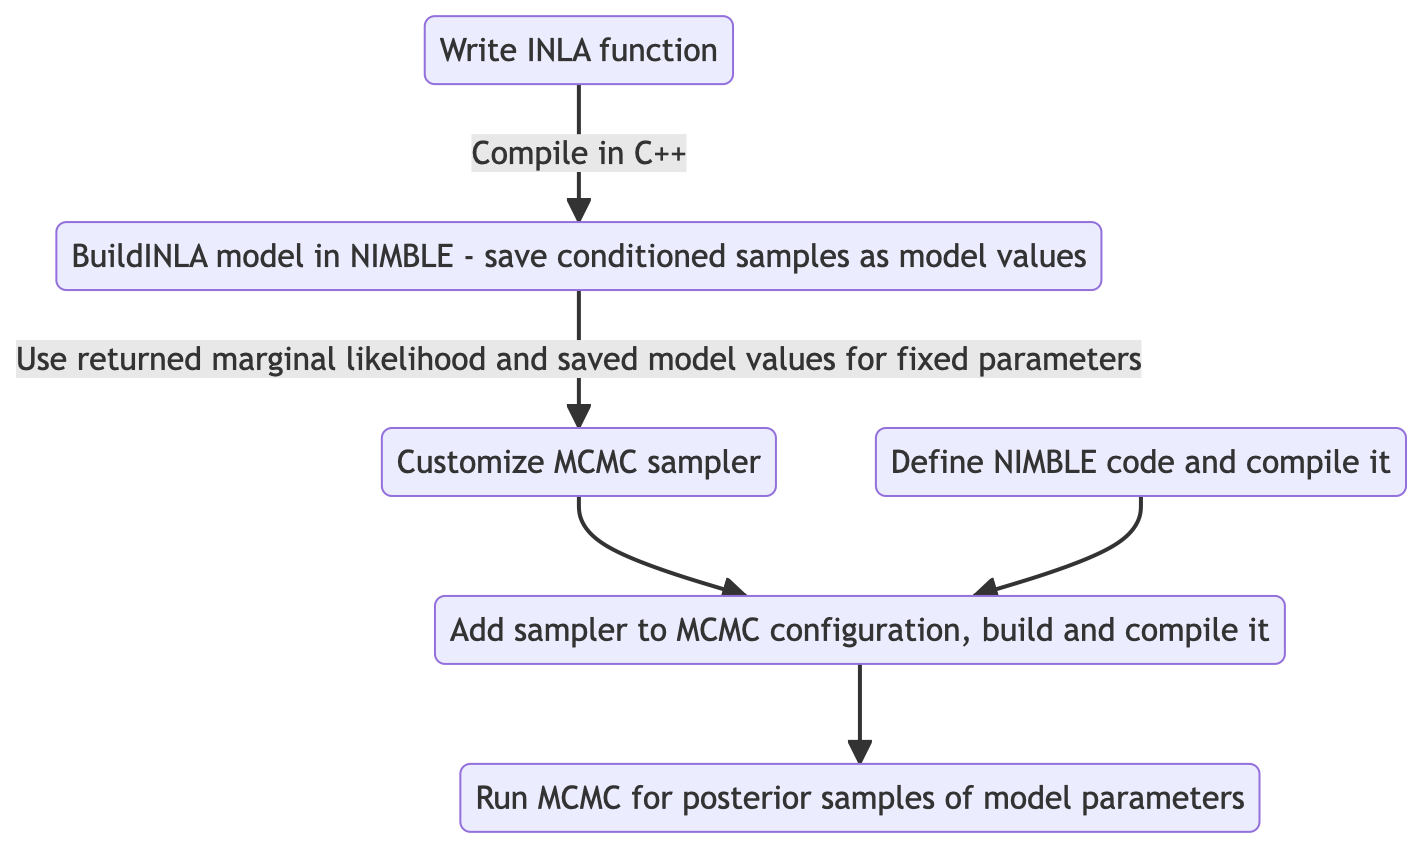
\includegraphics{flowxchartINLANimble.png}

}

\caption{\label{fig-flowchart}Flowchart showing how models can be fitted
using INLA\_MCMC framework implemented with NIMBLE. The process begins
by writing and compiling INLA model written as an R-function. Then a
NIMBLE model sampler is written to use the returned output from the INLA
function. This customised sampler is assigned to a compiled NIMBLE code
and MCMC is run to obtain posterior samples of all model parameters of
interest.}

\end{figure}

The random-walk block proposal is a Metropolis-Hastings algorithm, and
following the discussion by \citet{gomez2018markov}, proposal
distributions need to be chosen to propose new values of
\(\mathbf{z}_c\). This proposed value (say \(\mathbf{z}_c^{\star}\))
will be accepted or rejected with acceptance probability:
\begin{equation}\label{rwmhar}
\alpha = \text{min}\bigg \{ 1, \frac{\pi(\mathbf{y}| \mathbf{z}_{c}) \pi(\mathbf{z}_c^{\star}) q(\mathbf{z}_{c}^{(j)}| \mathbf{z}_c^{\star})}{\pi(\mathbf{y}| \mathbf{z}_{c}^{(j)})\pi(\mathbf{z}_c^{(j)}) q(\mathbf{z}_c^{\star}|\mathbf{z}_{c}^{(j)})}    \bigg \},
\end{equation} where \(q(.|.)\) is the proposal distribution;
\(\pi(\mathbf{y}| \mathbf{z}_{c}^{(j)})\) and
\(\pi(\mathbf{y}| \mathbf{z}_{c})\) are marginal distributions
approximated with \textbf{R-INLA}; and \(\pi(\mathbf{z}_c^{\star})\) and
\(\pi(\mathbf{z}_c)\) are the prior distributions of
\(\mathbf{z}_c^{\star}\) and \(\pi(\mathbf{z}_c)\) respectively.

For each step \(j\) of the MCMC, the conditional marginal distribution
on \(\mathbf{z}_{c}^{(j)}\) is approximated by integrating over
\(\mathbf{z}_{c}\): \begin{equation}\label{marginalzcmcmc}
\begin{split}
\pi(z_{-c,k}|\mathbf{y}) &= \int \pi(z_{-c,k}|\mathbf{z}_c, \mathbf{y})\pi(\mathbf{z}_c| \mathbf{y})d\mathbf{z}_c\\
&= \frac{1}{N} \sum_{j = 1}^{N} \pi(z_{-c,k}|\mathbf{z}^{j}_c, \mathbf{y}),
\end{split}
\end{equation} where \(N\) is the number of samples of the posterior
distribution of \(z_c\). This implies that the marginal of \(z_{-c,k}\)
can be obtained via Bayesian model averaging (BMA). In \textbf{R-INLA},
posterior estimates can be obtained from functions
\textit{inla.emarginal} (for posterior mean) and \textit{inla.zmarginal}
(for several other summary statistics). In this study, however, we draw
samples from the posterior distribution of \(z_{-c,k}\) from the fitted
conditional models using \textit{inla.samples} function in
\textbf{R-INLA} at each iteration.

Algorithm \ref{alg:altone} illustrates how the random walk block sampler
is customized to take into account the marginal likelihood and samples
from the posterior distribution of \(z_{-c,k}\) from \textbf{R-INLA}.

\begin{algorithm}
\caption{Metropolis Hastings with INLA using random walk block sampler}\label{alg:altone}
\begin{algorithmic}
\For{$i$ in $1:n.iter$ } 
  \If{i = 1}
  \State $\mathbf{z}_{c} := \mathbf{0} $
  \EndIf
\\
  \State Propose $\mathbf{z}_c^{\star} \sim N(0, \Sigma) $. \\
  \State Fit conditional model with $\mathbf{z}_c^{\star}$ as fixed values using $\textbf{R-INLA}$ and extract $\pi(\mathbf{y}| \mathbf{z}_{c})$ and a sample from the posterior distribution $pi(z_{-c}^{\star})$. \\
  \State Calculate acceptance probability with equation \eqref{rwmhar}. \\
  \State Generate $u \sim Uniform(0,1)$ \\
  \If{$\alpha < u$} 
  \State Set $\mathbf{z}_{c} := \mathbf{z}_c^{\star}$, $\pi(\mathbf{y}| \mathbf{z}_{c}) := \pi(\mathbf{y}| \mathbf{z}_{c}^{\star})$ and $\mathbf{z}_{-c} := \mathbf{z}_{-c}^{\star}$
  \Else 
  \State set $\mathbf{z}_{c} := \mathbf{z}_c$, $\pi(\mathbf{y}| \mathbf{z}_{c}) := \pi(\mathbf{y}| \mathbf{z}_{c}^{(i-1)})$ and $\mathbf{z}_{-c} := \mathbf{z}_{-c}^{i-1}$
  \EndIf
  
\EndFor
\end{algorithmic}
\end{algorithm}

\hypertarget{approach-two-writing-a-distribution-function-with-an-embedded-inla-function}{%
\subsection{\texorpdfstring{Approach two: Writing a distribution
function with an embedded INLA function
\label{alttwo}}{Approach two: Writing a distribution function with an embedded INLA function }}\label{approach-two-writing-a-distribution-function-with-an-embedded-inla-function}}

The first approach requires the user to have some competency in writing
algorithms in NIMBLE. Alternatively, we explored the option of writing a
NIMBLE distribution function that includes the \textbf{R-INLA}-defined
functions. The \textbf{R-INLA} function returns the conditional marginal
(\(\pi(y|\mathbf{z}_{c})\)) and samples of \(\mathbf{z}_{-c}\) from its
posterior distribution. The response variable \(\textbf{y}\) in the BUGS
code is assigned this written NIMBLE distribution. The BUGS code can
then be compiled, set up to run with MCMC configurations using the
sampling algorithms implemented in \textbf{nimble}, as shown in Figure
\ref{fig-flowchartAlt2}.

\begin{figure}

{\centering 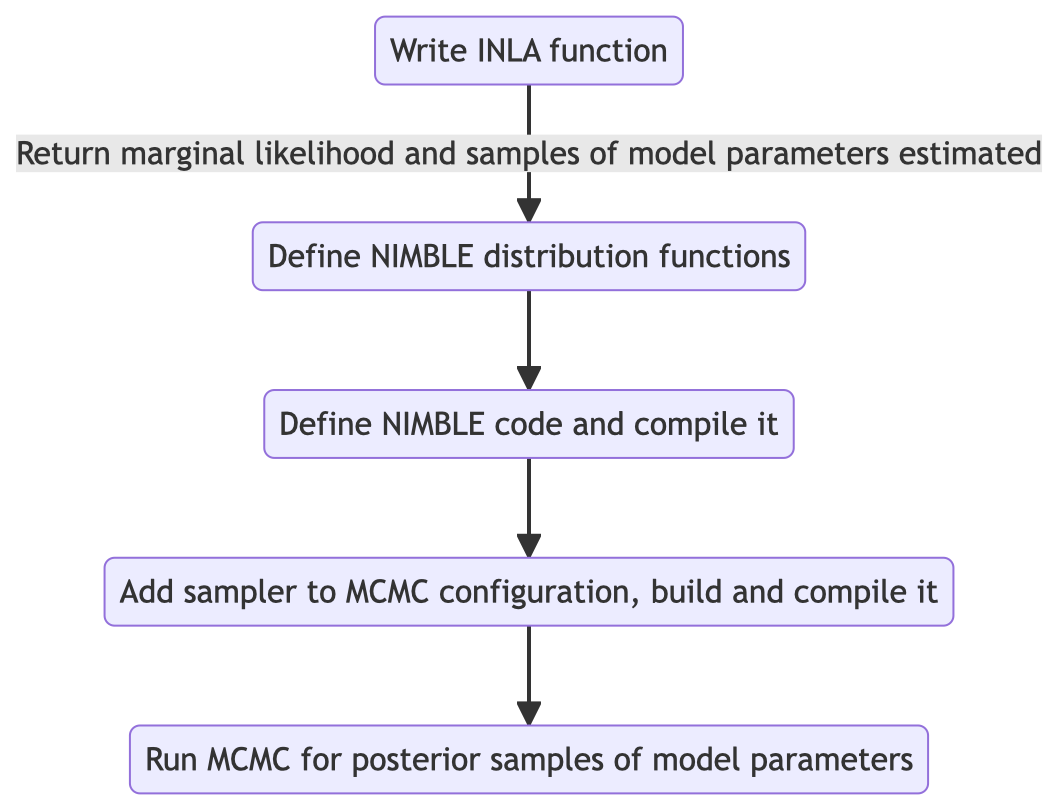
\includegraphics{flowxchartINLANimbleAlt2.png}

}

\caption{\label{fig-flowchartAlt2}Flowchart showing how models can be
fitted using INLA-MCMC methodology with alternative two. The process
begins by writing and compiling an \textbf{R-INLA} function that fits
the conditional model. New NIMBLE distributions that integrates the INLA
function are defined for use in BUGS code, and ths BUGS code is
configured to run in NIMBLE.}

\end{figure}

New distributions for use in BUGS code are set up for use in NIMBLE via
the \textit{registerDistributions} function in \textbf{nimble}
\citep[for further details on writing new distributions in NIMBLE, see Chapter 12.2 of ][]{nimblemanual}.
Here is a simple example to illustrate how the NIMBLE distribution can
be defined to integrate the \textbf{R-INLA} function.

\begin{Shaded}
\begin{Highlighting}[]
\CommentTok{\# Write conditional model to be fitted with INLA as a function}
\NormalTok{fitInla }\OtherTok{\textless{}{-}} \ControlFlowTok{function}\NormalTok{(beta, y, covariate)\{}
  \CommentTok{\#fit inla model}
\NormalTok{  res }\OtherTok{\textless{}{-}} \FunctionTok{inla}\NormalTok{(y }\SpecialCharTok{\textasciitilde{}} \DecValTok{1} \SpecialCharTok{+}\NormalTok{ beta}\SpecialCharTok{*}\NormalTok{covariate,}
\NormalTok{              ...)}
  \CommentTok{\#return marginal likelihood estimate}
\NormalTok{  mld }\OtherTok{\textless{}{-}}\NormalTok{ res}\SpecialCharTok{$}\NormalTok{mld[}\DecValTok{1}\NormalTok{,}\DecValTok{1}\NormalTok{]}
  \FunctionTok{return}\NormalTok{(mld)}
\NormalTok{\}}

\CommentTok{\# Convert the fitInla function to a NimbleFunction}
\NormalTok{nimbleINLA }\OtherTok{\textless{}{-}}\NormalTok{ nimble}\SpecialCharTok{::}\FunctionTok{nimbleRcall}\NormalTok{(}
  \AttributeTok{prototype =} \ControlFlowTok{function}\NormalTok{(}
 \AttributeTok{beta =} \FunctionTok{double}\NormalTok{(}\DecValTok{0}\NormalTok{), }\CommentTok{\#beta is a scalar}
 \AttributeTok{y =} \FunctionTok{double}\NormalTok{(}\DecValTok{1}\NormalTok{), }\CommentTok{\#y is a vector}
 \AttributeTok{x =} \FunctionTok{double}\NormalTok{(}\DecValTok{1}\NormalTok{) }\CommentTok{\#x is a vector}
\NormalTok{  ) \{\},}
  \AttributeTok{returnType =} \FunctionTok{double}\NormalTok{(}\DecValTok{0}\NormalTok{), }\CommentTok{\# outcome is a scalar}
  \AttributeTok{Rfun =} \StringTok{\textquotesingle{}fitInla\textquotesingle{}}
\NormalTok{)}
\CommentTok{\# Define density function}
\NormalTok{dINLA }\OtherTok{\textless{}{-}} \FunctionTok{nimbleFunction}\NormalTok{(}
  \AttributeTok{run =} \ControlFlowTok{function}\NormalTok{(}\AttributeTok{y =} \FunctionTok{double}\NormalTok{(}\DecValTok{1}\NormalTok{),}
                 \AttributeTok{beta =} \FunctionTok{double}\NormalTok{(}\DecValTok{0}\NormalTok{), }
                 \AttributeTok{covariate =} \FunctionTok{double}\NormalTok{(}\DecValTok{0}\NormalTok{),}
                 \AttributeTok{log =} \FunctionTok{logical}\NormalTok{(}\DecValTok{0}\NormalTok{, }\AttributeTok{default =} \DecValTok{0}\NormalTok{)) \{}
    \FunctionTok{returnType}\NormalTok{(}\FunctionTok{double}\NormalTok{())}
\CommentTok{\#run the INLA function and return marginal likelihood}
\NormalTok{    mld }\OtherTok{\textless{}{-}} \FunctionTok{nimbleINLA}\NormalTok{(beta, y,covariate)}
    \ControlFlowTok{if}\NormalTok{(log) }\FunctionTok{return}\NormalTok{(mld)}
    \FunctionTok{return}\NormalTok{(}\FunctionTok{exp}\NormalTok{(mld))}
\NormalTok{  \})}

\CommentTok{\#Register the distributions}
\FunctionTok{registerDistributions}\NormalTok{(}\FunctionTok{list}\NormalTok{(}
  \AttributeTok{dSpatial =} \FunctionTok{list}\NormalTok{(}
    \AttributeTok{BUGSdist =} \StringTok{"dINLA(beta, covariate)"}\NormalTok{,}
    \AttributeTok{discrete =} \ConstantTok{TRUE}\NormalTok{,}
    \AttributeTok{range =} \FunctionTok{c}\NormalTok{(}\SpecialCharTok{{-}}\ConstantTok{Inf}\NormalTok{, }\ConstantTok{Inf}\NormalTok{),}
    \AttributeTok{types =} \FunctionTok{c}\NormalTok{(}\StringTok{\textquotesingle{}value = double(1)\textquotesingle{}}\NormalTok{, }\StringTok{\textquotesingle{}covariate = double(1)\textquotesingle{}}\NormalTok{, }\StringTok{\textquotesingle{}beta = double(0)\textquotesingle{}}\NormalTok{)}
\NormalTok{  )))}
\end{Highlighting}
\end{Shaded}

\hypertarget{examples}{%
\section{Examples}\label{examples}}

We illustrate the proposed method with six examples. The first two
examples are simulation studies on bivariate regression model from
\citet{gomez2018markov} and spatial occupancy model from
\citet{kery2020applied}. The method was also applied to four models with
datasets: Bayesian lasso regression with \textit{Hitters} dataset
\citep{gareth2013introduction}, imputation of missing covariates with
\textit{nhanes} dataset accessed from the R-package \textbf{mice}
\citep{van2011mice}, zero-inflated Poisson model and Binomial N-Mixture
model with mallard data \citep{unmarked}.

The various models are fitted with the proposed methodology described in
section \ref{inlamcmc}. Specifically. we fit approach one (described in
section \ref{altone}) with the customized RW-block samplers (referred to
as \texttt{iNim-RW} in the rest of this paper). In addition, we fit
approach two (described in section \ref{alttwo}) with \textbf{nimble}'s
implemented RW\_block sampler assigned to \(\mathbf{z}_{c}\) (we refer
to this approach as \texttt{iNim2-RW} in the rest of this paper ). We
also fit bivariate regression model with \textbf{R-INLA}, the lasso
regression with the R-package \textbf{glmnet} \citep{glmnet}, the
zero-inflated Poisson regression with \textbf{pscl}\citep{pscl} and the
Binomial N-mixture model with R-package \textbf{unmarked}
\citep{unmarked} to compare with the results we obtain from the proposed
framework. To assess the performance of the various approaches, the
efficiency of each method is estimated. The efficiency is calculated as
the effective sample size divided by the time used to generate the
samples. The effective sample size was estimated with the R-package
\textbf{mcmcse} \citep{mcmcse}.

For all models fitted with NIMBLE, one chain is run for \(100500\)
iterations and the first \(50500\) samples are discarded as burn-in
samples. We keep every fifth of the remaining samples for inference.

\hypertarget{simulation-study}{%
\subsection{Simulation Study}\label{simulation-study}}

\hypertarget{bivariate-regression-model}{%
\subsubsection{Bivariate regression
model}\label{bivariate-regression-model}}

We use the simulation study on Bivariate regression model in
\citet{gomez2018markov} as our first example. The aim of the simulation
is to compare the marginal distribution of model parameters and joint
posterior distribution of the covariate effect parameters estimated from
the fitted model using INLA, MCMC and INLA-MCMC methods.

We simulate \(100\) observations with two covariates \(\mathbf{u_1}\)
and \(\mathbf{u_2}\) as follows:
\begin{equation}\label{bivariateRegression}
y_i = \alpha + \beta_1 u_{1i} + \beta_2 u_{2i} + \epsilon_i; \quad i = 1, \ldots, 100
\end{equation} where \(\mathbf{u_1}\) and \(\mathbf{u_2}\) are simulated
from uniform distribution between 0 and 1, and \(\epsilon_i\) is a
Gaussian random term with mean zero and variance \(1/\tau\). Moreover,
we choose \(\alpha = 2\), \(\beta_1 = 3\), \(\beta_2 = -3\) and
\(\tau=1\).

As noted by both \citet{gomez2018markov} and
\citet{berild2022importance}, INLA can easily fit this model. We split
the entire parameters in the model
\(\mathbf{z} = \{\alpha ,\beta_1, \beta_2, \tau \}\) into two mutually
exclusive sets: \(\mathbf{z}_c = \{\beta_1, \beta_2 \}\) and
\(\mathbf{z}_{-c} = \{\alpha, \tau \}\), similar to what was done by
\citet{gomez2018markov} and \citet{berild2022importance}. New samples of
\(\mathbf{z}_c\) are proposed from a multivariate normal distribution
with zero mean and covariance matrix \(\Sigma = 0.75^2 I\), where \(I\)
is an identity matrix.

\begin{figure}

{\centering 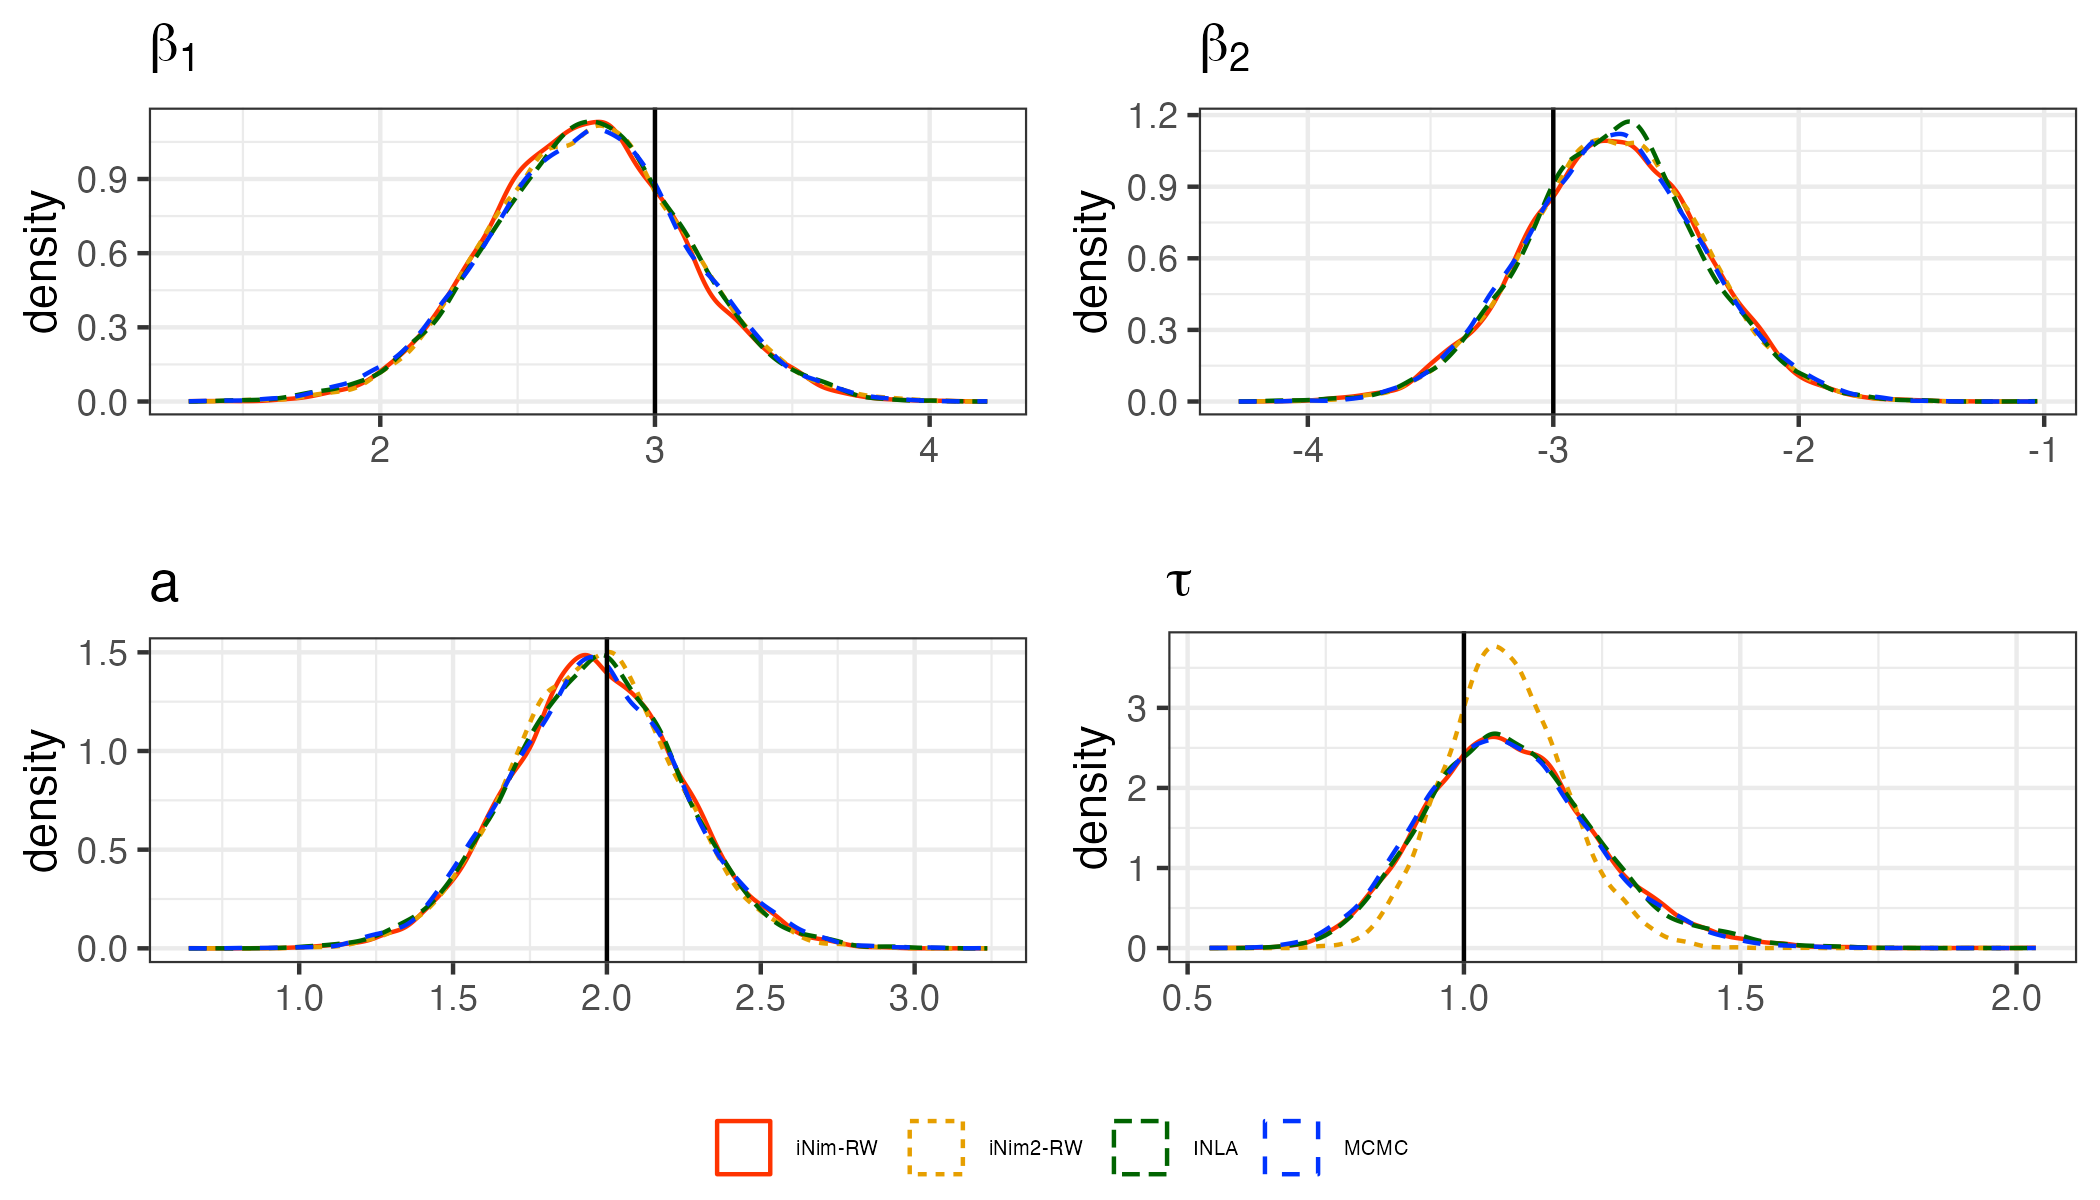
\includegraphics{results/bivariateRegression.png}

}

\caption{\label{fig-bivariatePlot}Posterior marginal distribution of the
parameters in the bivariate regression model. The distributions are
coloured by the method used to fit the model and the solid vertical line
represents the true model parameter value used to simulate the data.}

\end{figure}

\begin{figure}

{\centering 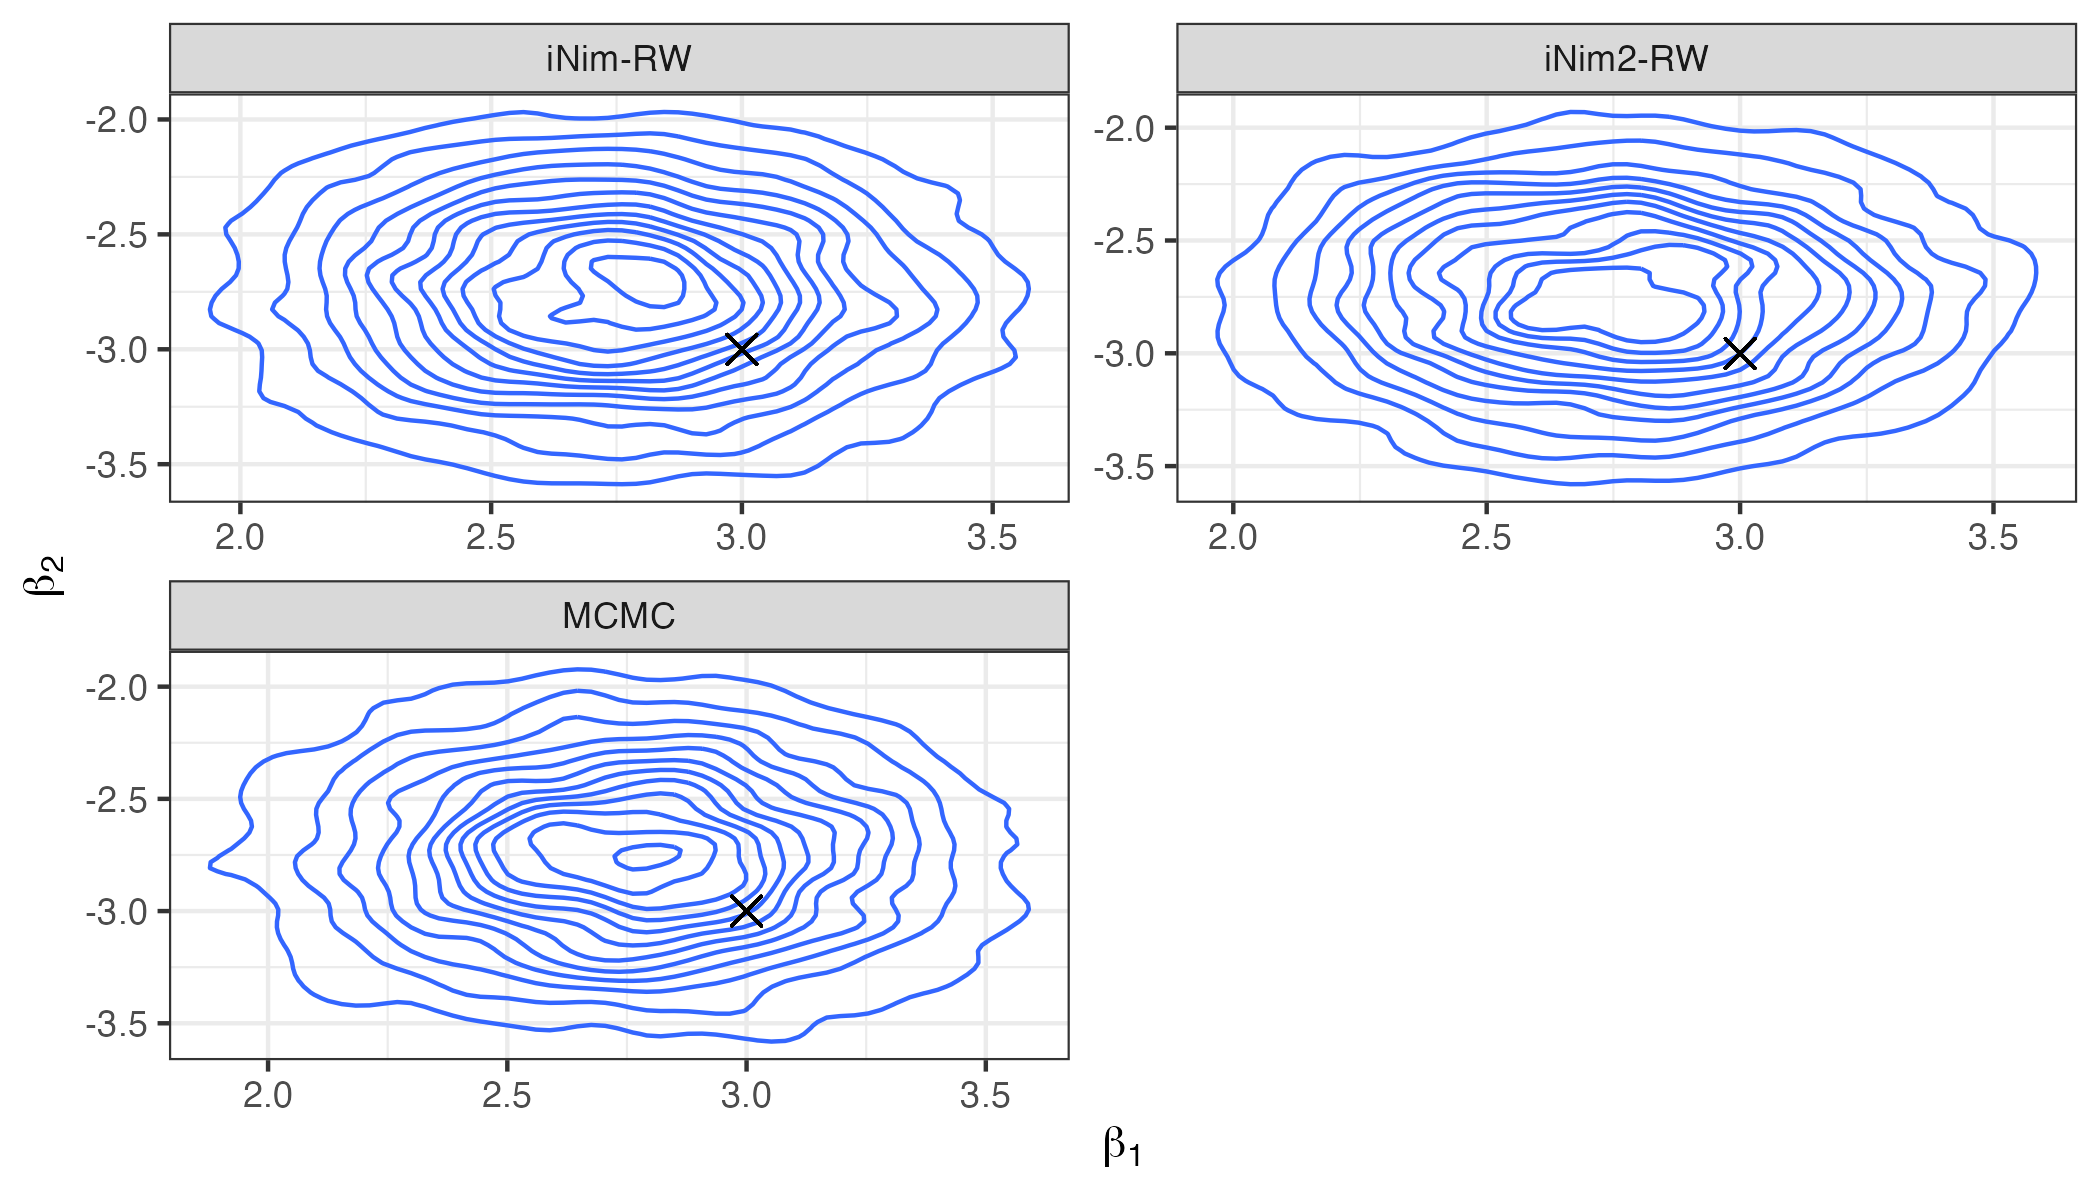
\includegraphics{results/bivariateContour.png}

}

\caption{\label{fig-bivariateContour}Joint posterior distribution of the
covariate effects \(\beta_1\) and \(\beta_2\) from the bivariate
regression model. The true value is indicated with the black cross.}

\end{figure}

Figure \ref{fig-bivariatePlot} shows the marginal distributions of the
four model parameters in the bivariate regression model defined in
equation \eqref{bivariateRegression}, with the joint distribution of
\(\beta_1\) and \(\beta_2\) presented in Figure
\ref{fig-bivariateContour}. The effective sample sizes and time taken
for the model to be fitted with each study method is presented in Table
\ref{tbl-bivariateESS}. In all cases, the posterior marginals of the
model parameters are very similar. Moreover, the effective sample size
is higher for the first approach (iNim-RW) than the second approach
(iNim2-RW) and MCMC. This implies that to achieve the same number of
independent observations from the posterior distribution, iNim-RW would
require less iterations to do that.

Although iNim-RW, iNim2-RW and MCMC methods were compiled and run in
C++, MCMC with \textbf{nimble} was the fastest in this example (2.87
seconds). Fitting the conditional model with \textbf{R-INLA} is very
fast, however the implementation of the INLA-MCMC approaches with NIMBLE
calls the \textbf{R-INLA} sequentially. As a result, iNim-RW and
iNim2-RW took over \(37\) hours to run for \(100500\) iterations. This
long computational time of the INLA-MCMC method has also been noted by
\cite{berild2022importance}.

\hypertarget{tbl-bivariateESS}{}
\begin{longtable}{llll}
\caption{\label{tbl-bivariateESS}Effective sample size (with efficiency provided in parenthesis) of each
model parameter and time taken by each of the methods in the study.
Efficiency is calculated as the effective sample size divided by the
computational time. }\tabularnewline

\toprule
Parameter & iNim-RW & iNim2-RW & MCMC\\
\midrule
\endfirsthead
\multicolumn{4}{@{}l}{\textit{(continued)}}\\
\toprule
Parameter & iNim-RW & iNim2-RW & MCMC\\
\midrule
\endhead

\endfoot
\bottomrule
\endlastfoot
\cellcolor{gray!15}{$\alpha$} & \cellcolor{gray!15}{5094.29 (0.02)} & \cellcolor{gray!15}{4316.95 (0.02)} & \cellcolor{gray!15}{688.6 (313.42)}\\
$\beta_1$ & 5143.61 (0.02) & 4487.63 (0.02) & 1140.77 (519.22)\\
\cellcolor{gray!15}{$\beta_2$} & \cellcolor{gray!15}{5741.92 (0.02)} & \cellcolor{gray!15}{4787.93 (0.02)} & \cellcolor{gray!15}{975.87 (444.17)}\\
$\tau$ & 5970.26 (0.02) & 7744.35 (0.04) & 10000 (4551.5)\\*
\end{longtable}

\hypertarget{spatial-occupancy-model}{%
\subsubsection{\texorpdfstring{Spatial Occupancy model
\label{spatialOccupancyModel}}{Spatial Occupancy model }}\label{spatial-occupancy-model}}

Inference and predictions of species occupancy is an essential part of
ecological and conservation studies. To make such inferences and
predictions about species occupancy, species distribution models are
fitted to biodiversity data with species presence and absence
information whilst accounting for imperfect detection. These fitted
species distribution models can include random effects that capture the
spatial autocorrelation in the data. This spatial autocorrelation can be
caused by either accidentally omitting spatial covariates in the model
or because the data contains biotic processes such as dispersal and
conspecific attraction \citep{kery2020applied}.

In ecological problems, these models are usually fitted with MCMC;
however they can be very data-rich and computationally expensive to fit
with MCMC \citep{kery2020applied}. Specialized R-packages for particular
classes of models like \textbf{spBayes} \citep{spBayes} and
\textbf{R-INLA} as well as custom written MCMC engines like NIMBLE, Stan
\citep{carpenter2017stan} can be used for such complex problems
\citep{kery2015applied}. The disadvantage of using \textbf{spBayes} and
\textbf{R-INLA} is that it is not possible to incorporate imperfect
detection and false positives in the species distribution models
\citep{kery2020applied}. Here, we use the INLA-MCMC method to fit
spatial occupancy model that accounts for imperfect detection to a
simulated dataset. We do this by sampling the observation model
parameters and the true species occupancy state from MCMC and the
ecological process model with the R-package \textbf{inlabru}
\citep{bachl2019inlabru}, a wrapper around \textbf{R-INLA}.

We simulate data for a static occupancy model with residual spatial
autocorrelation in occupancy probability using the function
\textit{simOCCSpatial} in the R-package \textbf{AHMbook}
\citep{ahmbook}. The function generates occupancy data with a negative
exponential autocorrelation function for the Gaussian random field plus
a linear and quadratic effect of elevation on the occupancy probability
and negative effects of forest cover and wind-speed on detection
probability. See Chapter 9.4 of \citet{kery2020applied} for details of
the simulation function. The data was simulated for \(50\) sites and
\(10\) survey visits.

The model we aim to fit and the prior distributions assigned to the
hyperparameters are as follows: \begin{equation}
\begin{split}
logit(\psi_i) &= \beta_0 + \beta_1 elev_{i} + \beta_2 elev_{i}^{2} + \eta_i, \quad \text{where $\eta_i \sim N(\mathbf{0}, \mathbb{\Sigma})$} \\
\zeta_i &\sim Bernoulli (\psi_i)\\
logit(p_{ij}) &= \alpha_0 + \alpha_1 forestCover_{i} + \alpha_2 wind_{ij}\\
y_{ij} &\sim Bernoulli(\zeta_i \times p_{ij})\\
\text{Prior distributions:}\\
\alpha_0, \alpha_1, \alpha_2 &\sim N(0, 0.0001) \\
\beta_0, \beta_1, \beta_2 &\sim N(0, 0.0001)\\
\end{split}
\end{equation} where \(\mathbb{\Sigma}\) is the variance covariance
matrix of the site effect, defined in terms of a constant variance
parameter \(\sigma^2\) and an exponential decay parameter \(\theta\),
\(\zeta_i\) is the latent occupancy state at site \(i\), \(\psi_i\) is
the occupancy probability at site \(i\) and \(p_{ij}\) is the detection
probability at site \(i\) during survey visit \(j\).

The parameters and latent state \(\zeta\) in the model
\(\mathbf{z} = \{\alpha_0,\alpha_1,\alpha_2, \theta, \sigma^2, \zeta_1, \ldots, \zeta_{50} \}\)
into two mutually exclusive sets:
\(\mathbf{z}_c = \{\alpha_0,\alpha_1,\alpha_2, \zeta_1, \ldots, \zeta_{50} \}\)
and
\(\mathbf{z}_{-c} = \{\theta, \sigma^2, \beta_1, \beta_2, \beta_3 \}\).
New samples of \(\alpha_0,\alpha_1,\alpha_2\) are proposed from a
multivariate normal distribution with zero mean and covariance matrix
\(\Sigma = I\), where \(I\) is an identity matrix, and the latent state
parameter \(\zeta_1, \ldots, \zeta_{50}\) are sampled using
\textbf{nimble}'s default binary sampling algorithm. Posterior samples
of \(\mathbf{z}_{-c}\) are obtained from fitting a spatial regression
model with \(\zeta\) as the response variable.

\hypertarget{tbl-spatialOccupancy}{}
\begin{longtable}{llll}
\caption{\label{tbl-spatialOccupancy}Summary of spatial occupancy model parameters (with standard error in
paranthesis). The parameter \(\psi_{fs}\) is the realised occupancy
calculated as the average occupancy over all the study sites. }\tabularnewline

\toprule
Parameter & Truth & iNim-RW & MCMC\\
\midrule
\endfirsthead
\multicolumn{4}{@{}l}{\textit{(continued)}}\\
\toprule
Parameter & Truth & iNim-RW & MCMC\\
\midrule
\endhead

\endfoot
\bottomrule
\endlastfoot
\cellcolor{gray!15}{$\alpha_1$} & \cellcolor{gray!15}{-1} & \cellcolor{gray!15}{-0.7701 (0.2005)} & \cellcolor{gray!15}{-0.8026 (0.1775)}\\
$\alpha_2$ & 1 & 0.8842 (0.1845) & 0.9704 (0.1784)\\
\cellcolor{gray!15}{$\alpha_0$} & \cellcolor{gray!15}{-0.45} & \cellcolor{gray!15}{-0.6537 (0.2079)} & \cellcolor{gray!15}{-0.4912 (0.1511)}\\
$\beta_1$ & 2 & 0.0954 (0.9975) & 1.3966 (2.9925)\\
\cellcolor{gray!15}{$\beta_2$} & \cellcolor{gray!15}{-2} & \cellcolor{gray!15}{0.8111 (1.4912)} & \cellcolor{gray!15}{-0.6083 (2.181)}\\
$\beta_0$ & 2.197 & 1.7398 (0.865) & 0.655 (1.5259)\\
\cellcolor{gray!15}{$\psi_{fs}$} & \cellcolor{gray!15}{0.4664} & \cellcolor{gray!15}{0.52 (0.1381)} & \cellcolor{gray!15}{0.52 (0.0245)}\\*
\end{longtable}

The true parameter values and summaries of their posterior distribution
estimated from iNim-RW, iNim2-RW and MCMC are presented in Table
\ref{tbl-spatialOccupancy}. At the time of writing this manuscript, the
MCMC chains had been run for \(1000\) iterations. The MCMC results are
less biased than the INLA-MCMC results. Longer chains may produce
comparable results.

\hypertarget{application-to-real-datasets}{%
\subsection{Application to real
datasets}\label{application-to-real-datasets}}

\hypertarget{bayesian-lasso}{%
\subsubsection{Bayesian Lasso}\label{bayesian-lasso}}

The third example is taken from \citet{gomez2018markov}. The lasso
performs variable selection and model fitting at the same time by
providing estimates that are zero \citep{hastie2009introduction}. Lasso
tries to estimate coefficients of a model with a Gaussian likelihood by
minimizing:

\begin{equation}
\sum_{i = 1}^{N} \bigg( y_i - \alpha - \sum_{j = 1}^{n_{\beta}} \beta_j x_{ji} \bigg)^2 + \lambda \sum_{j = 1}^{n_{\beta}}|\beta_j|,
\end{equation} where \(y_i\) is the response variable, \(x_{ji}\) are
covariates with covariate effect \(\beta_j\) and \(n_{\beta}\) is the
number of covariates. The shrinkage of the coefficients is controlled by
the parameter \(\lambda\), with higher values of \(\lambda\) shrinking
the parameters to zero.

The Lasso regression can be used for Bayesian inference by fitting a
standard regression model with Laplace priors on the model coefficients.
The Laplace distribution is defined as: \begin{equation}
f(\beta) = \frac{1}{2 \sigma} exp \bigg(- \frac{|\beta - \mu|}{\sigma}  \bigg)
\end{equation} where the location and scale parameter is \(\mu\) and
\(\sigma\) respectively. The scale parameter is related to the shrinkage
parameter as \(\sigma = 1/\tau\). Currently \textbf{R-INLA} does not
have a Laplace prior distribution implemented as part of its latent
field. Hence, we use \textbf{R-INLA} to fit a Lasso regression model
conditioned on the parameters \(\beta\).

The Bayesian lasso model is fitted to the \textit{Hitters} dataset
described in \citet{gareth2013introduction}. The dataset contains
statistics about players in the Major league baseball. We aim to predict
the salary of players based on five covariates: number of times at bat,
number of hits, number of home runs, number of runs and number of runs
batted in. Player \(i\)'s salary (\(y_i\)) is assumed to be Gaussian
distributed with mean \(\beta_0 + \sum_{i=1}^{p} \beta_{p} x_{ij}\) and
precision \(\tau\), where \(\beta_{p}\) are covariate effects and
\(\beta_0\) is the intercept of the model.

We assumed a multivariate Gaussian with mean zero and covariance matrix
\(0.25(\textbf{X}^T\textbf{X})^{-1}\) as the proposal distribution on
the covariate coefficients
\(\mathbf{\beta} = \{\beta_1, \beta_2, \ldots, \beta_p \}\), where
\(\textbf{X}\) is a matrix with covariates as its columns.
\cite{gomez2018markov} and \cite{berild2022importance} noted this
proposal distribution yields good acceptance rates for the random-walk
samplers. Moreover, the prior on \(\tau\) is assumed to be Gamma
distributed with parameters \(1\) and \(5e^{-5}\), and intercept
\(\beta_0 \propto 1\).

\begin{figure}

{\centering 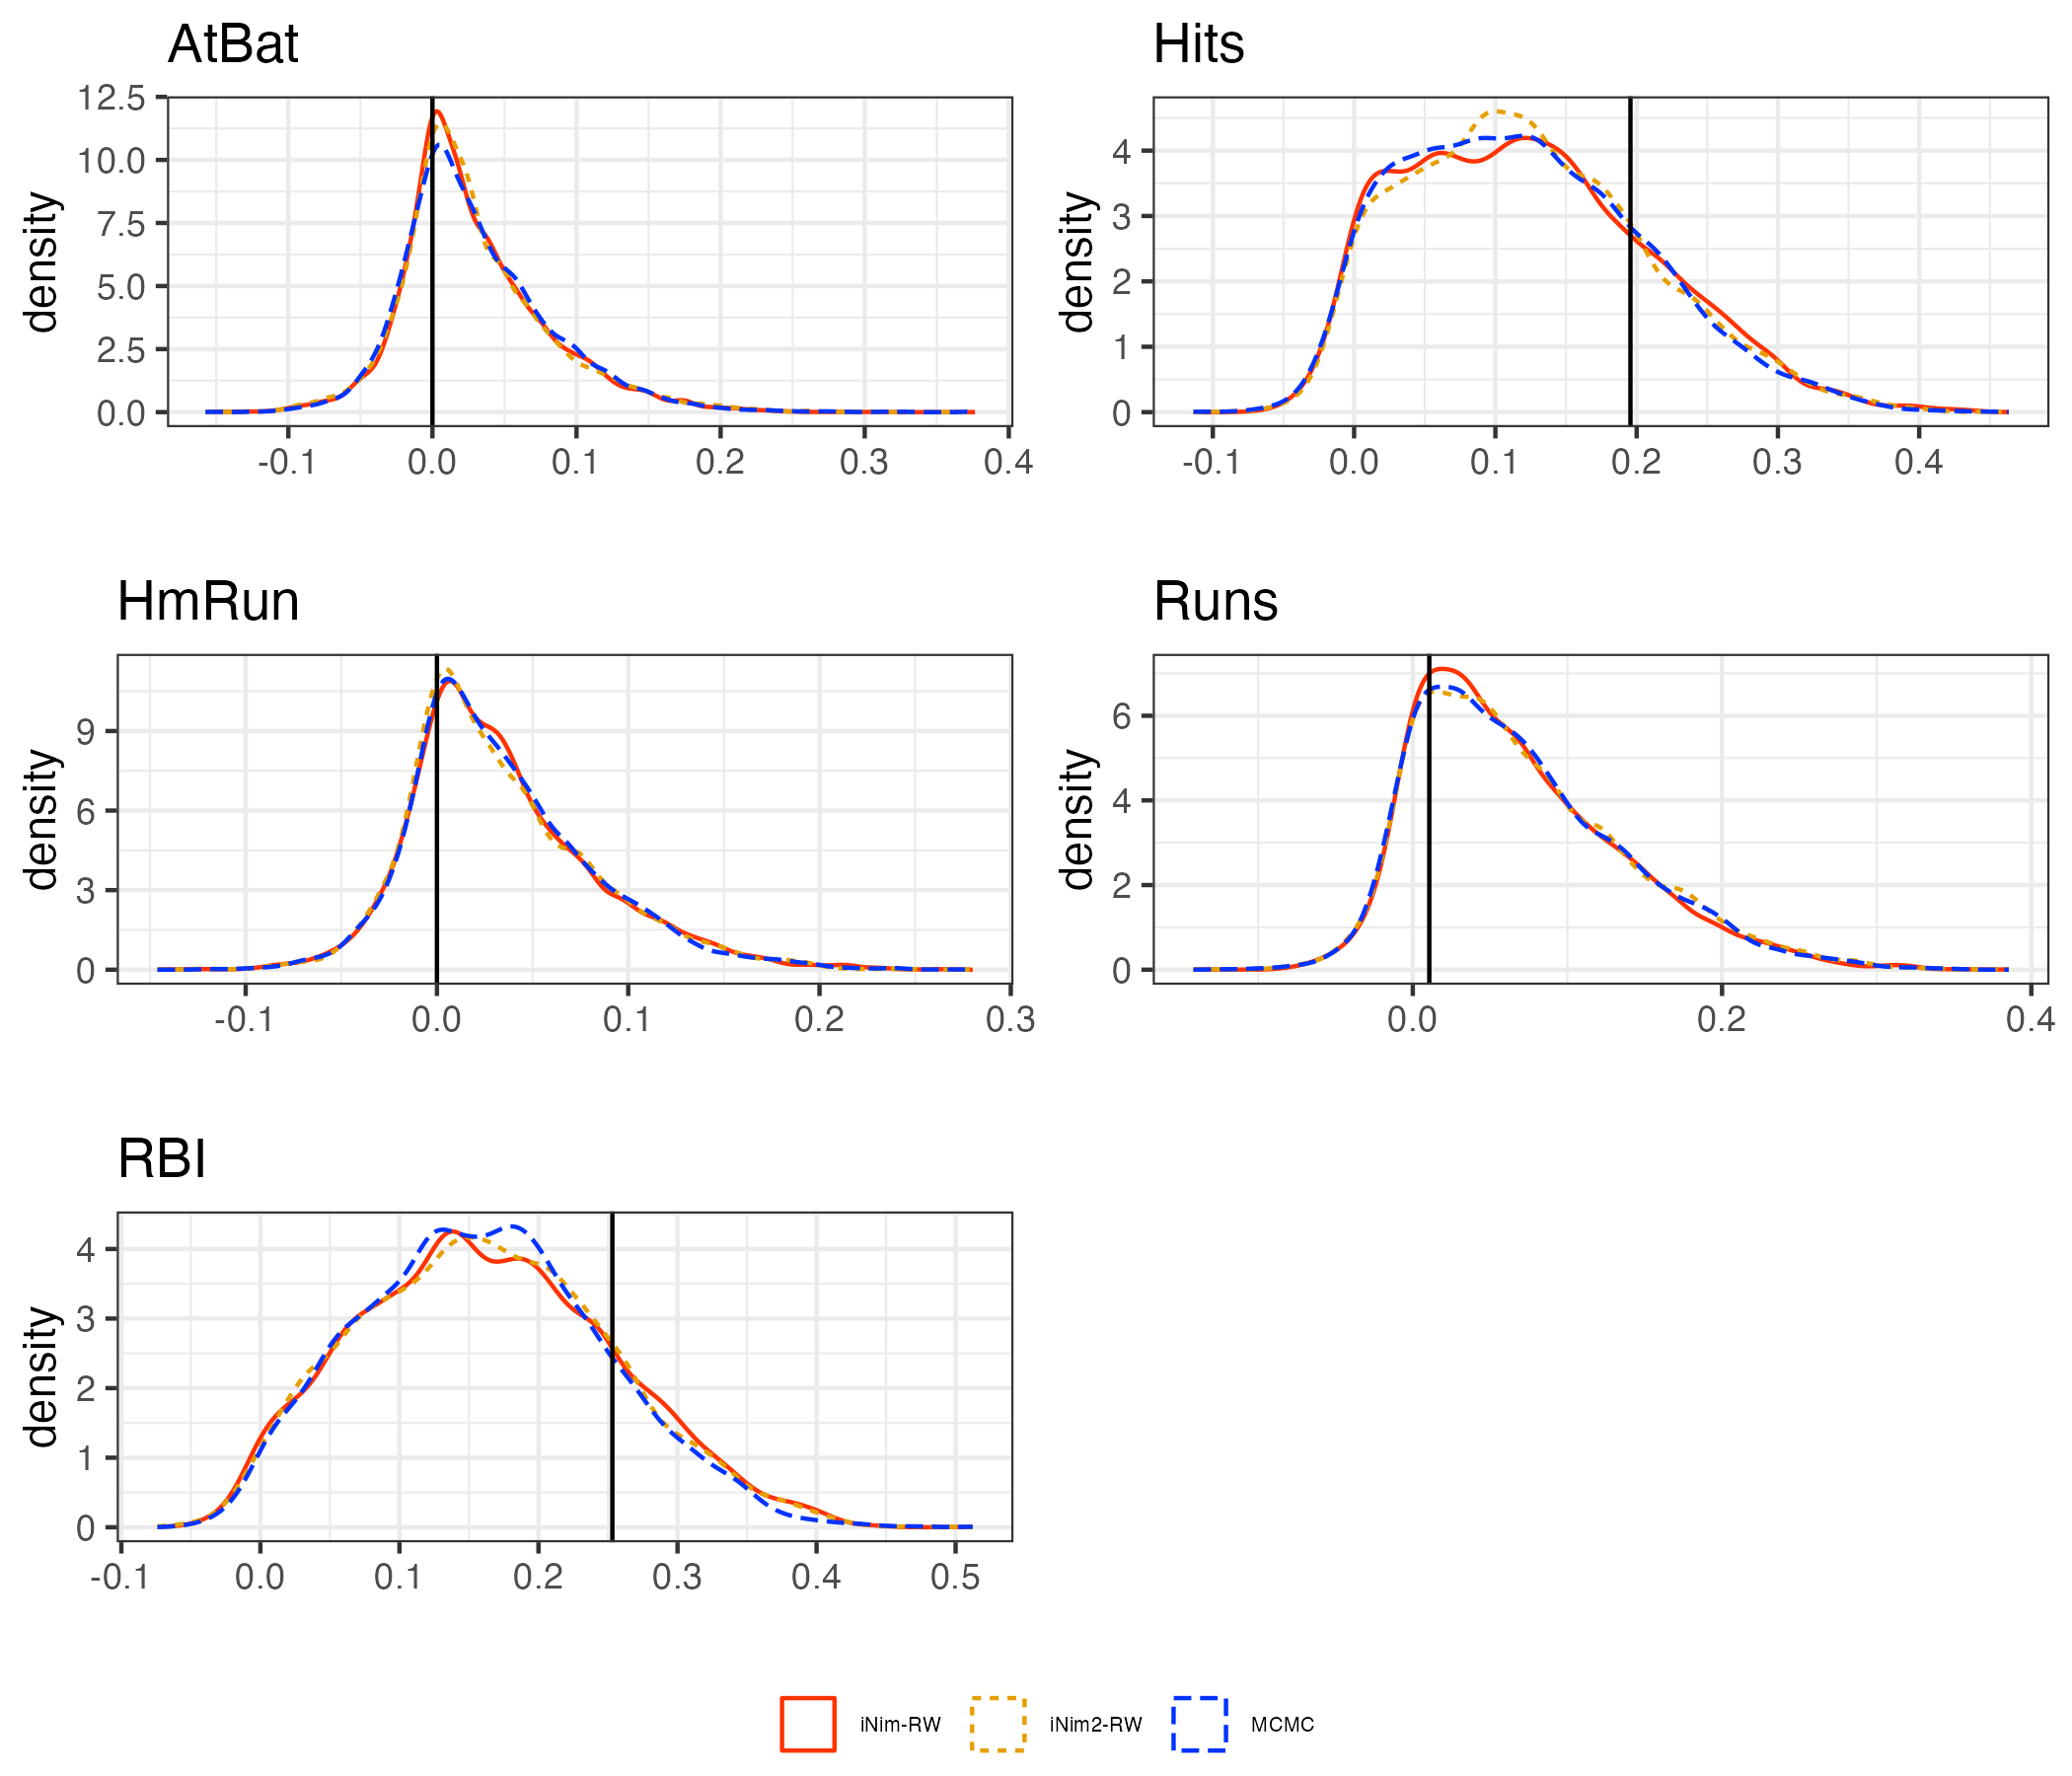
\includegraphics{results/lassoRegression.png}

}

\caption{\label{fig-lassoPlot}Posterior marginals of Lasso regression
model parameters obtained from MCMC and the INLA-MCMC approaches. The
solid vertical line indicates the maximum likelihood estimate of the
model parameters estimated with the R-package \textbf{glmnet}.}

\end{figure}

\hypertarget{tbl-lassoCovs}{}
\begin{longtable}{llllr}
\caption{\label{tbl-lassoCovs}Summary estimates of Lasso estimated with the R-package \textbf{glmnet}
and posterior mean from Bayesian Lasso (with standard deviation in
paranthesis) using the MCMC and INLA-MCMC approaches. }\tabularnewline

\toprule
Coefficient & iNim-RW & iNim2-RW & MCMC & Lasso\\
\midrule
\endfirsthead
\multicolumn{5}{@{}l}{\textit{(continued)}}\\
\toprule
Coefficient & iNim-RW & iNim2-RW & MCMC & Lasso\\
\midrule
\endhead

\endfoot
\bottomrule
\endlastfoot
\cellcolor{gray!15}{$\beta_1$} & \cellcolor{gray!15}{0.03 (0.05)} & \cellcolor{gray!15}{0.03 (0.05)} & \cellcolor{gray!15}{0.03 (0.03)} & \cellcolor{gray!15}{0.00}\\
$\beta_2$ & 0.12 (0.09) & 0.12 (0.08) & 0.12 (0.12) & 0.20\\
\cellcolor{gray!15}{$\beta_3$} & \cellcolor{gray!15}{0.03 (0.05)} & \cellcolor{gray!15}{0.03 (0.05)} & \cellcolor{gray!15}{0.03 (0.03)} & \cellcolor{gray!15}{0.00}\\
$\beta_4$ & 0.07 (0.07) & 0.07 (0.07) & 0.07 (0.07) & 0.01\\
\cellcolor{gray!15}{$\beta_5$} & \cellcolor{gray!15}{0.16 (0.09)} & \cellcolor{gray!15}{0.16 (0.09)} & \cellcolor{gray!15}{0.16 (0.16)} & \cellcolor{gray!15}{0.25}\\*
\end{longtable}

The posterior marginals of Lasso regression parameters are presented in
Figure \ref{fig-lassoPlot} and summary statistics of the posterior
marginals are presented in Table \ref{tbl-lassoCovs}. The posterior
marginals of \(\beta\) estimated from MCMC are comparable to those from
the INLA-MCMC methods. For the parameters with Lasso coefficients of
\(0\), the posterior distributions were centered around \(0\).

\hypertarget{imputation-of-missing-covariates}{%
\subsubsection{Imputation of missing
covariates}\label{imputation-of-missing-covariates}}

There are different multiple imputation methods that are available for
missing covariates, with several of them implemented in the R-package
\textbf{mice} \citep{van2011mice}. This example uses the \textit{nhanes}
dataset in the \textbf{mice} package which contains information on age
(\texttt{age} ), body mass index (\texttt{bmi}), hypertension status
(\texttt{hyp}) and cholesterol level (\texttt{chl}) of individuals from
a study. The values of age are completely observed, but there are
missing values in the body mass index and cholesterol level. Out of the
nine missing values in the body mass index, six of them have missing
cholesterol level values. The aim of this illustration, similar to that
of \citet{gomez2018markov}, is to impute the missing values in body mass
index and predict the cholesterol level through age and body mass index
by fitting a multiple linear regression model defined in equation
\eqref{missingCovariatesEquation}.

Until recently, \textbf{R-INLA} could not handle missing variables in
covariates \citep{gomez2018markov, berild2022importance}.
\cite{skarstein2023joint} has shown how to fit models with missing
covariates in \textbf{R-INLA}. We proceed with this example assuming
that the multivariate regression model cannot be fitted with
\textbf{R-INLA} unless the missing covariates are imputed.

The imputation method employed in this example uses a Gaussian prior for
the missing values of body mass index. The prior distribution is
centered around the mean of the observed values (\(26.56\)) and its
variance four times that of the observed values (\(71.07\)), similar to
what \citet{gomez2018markov} did.

The model we aim to fit is as follows:

\begin{equation}\label{missingCovariatesEquation}
\begin{split}
chl_i &= \beta_{0} + \beta_{1}\text{bmi}_i + \beta_{2}\text{age2}_i + \beta_{3}\text{age3}_i \\
\beta_0 & \propto 1 \\
\beta_k & \propto N(0, 0.0001); \quad k = 1, 2, 3 \\
\epsilon & \sim N(0, \tau)\\
\tau & \sim Ga(1, 0.00005)
\end{split}
\end{equation}

\begin{figure}

{\centering 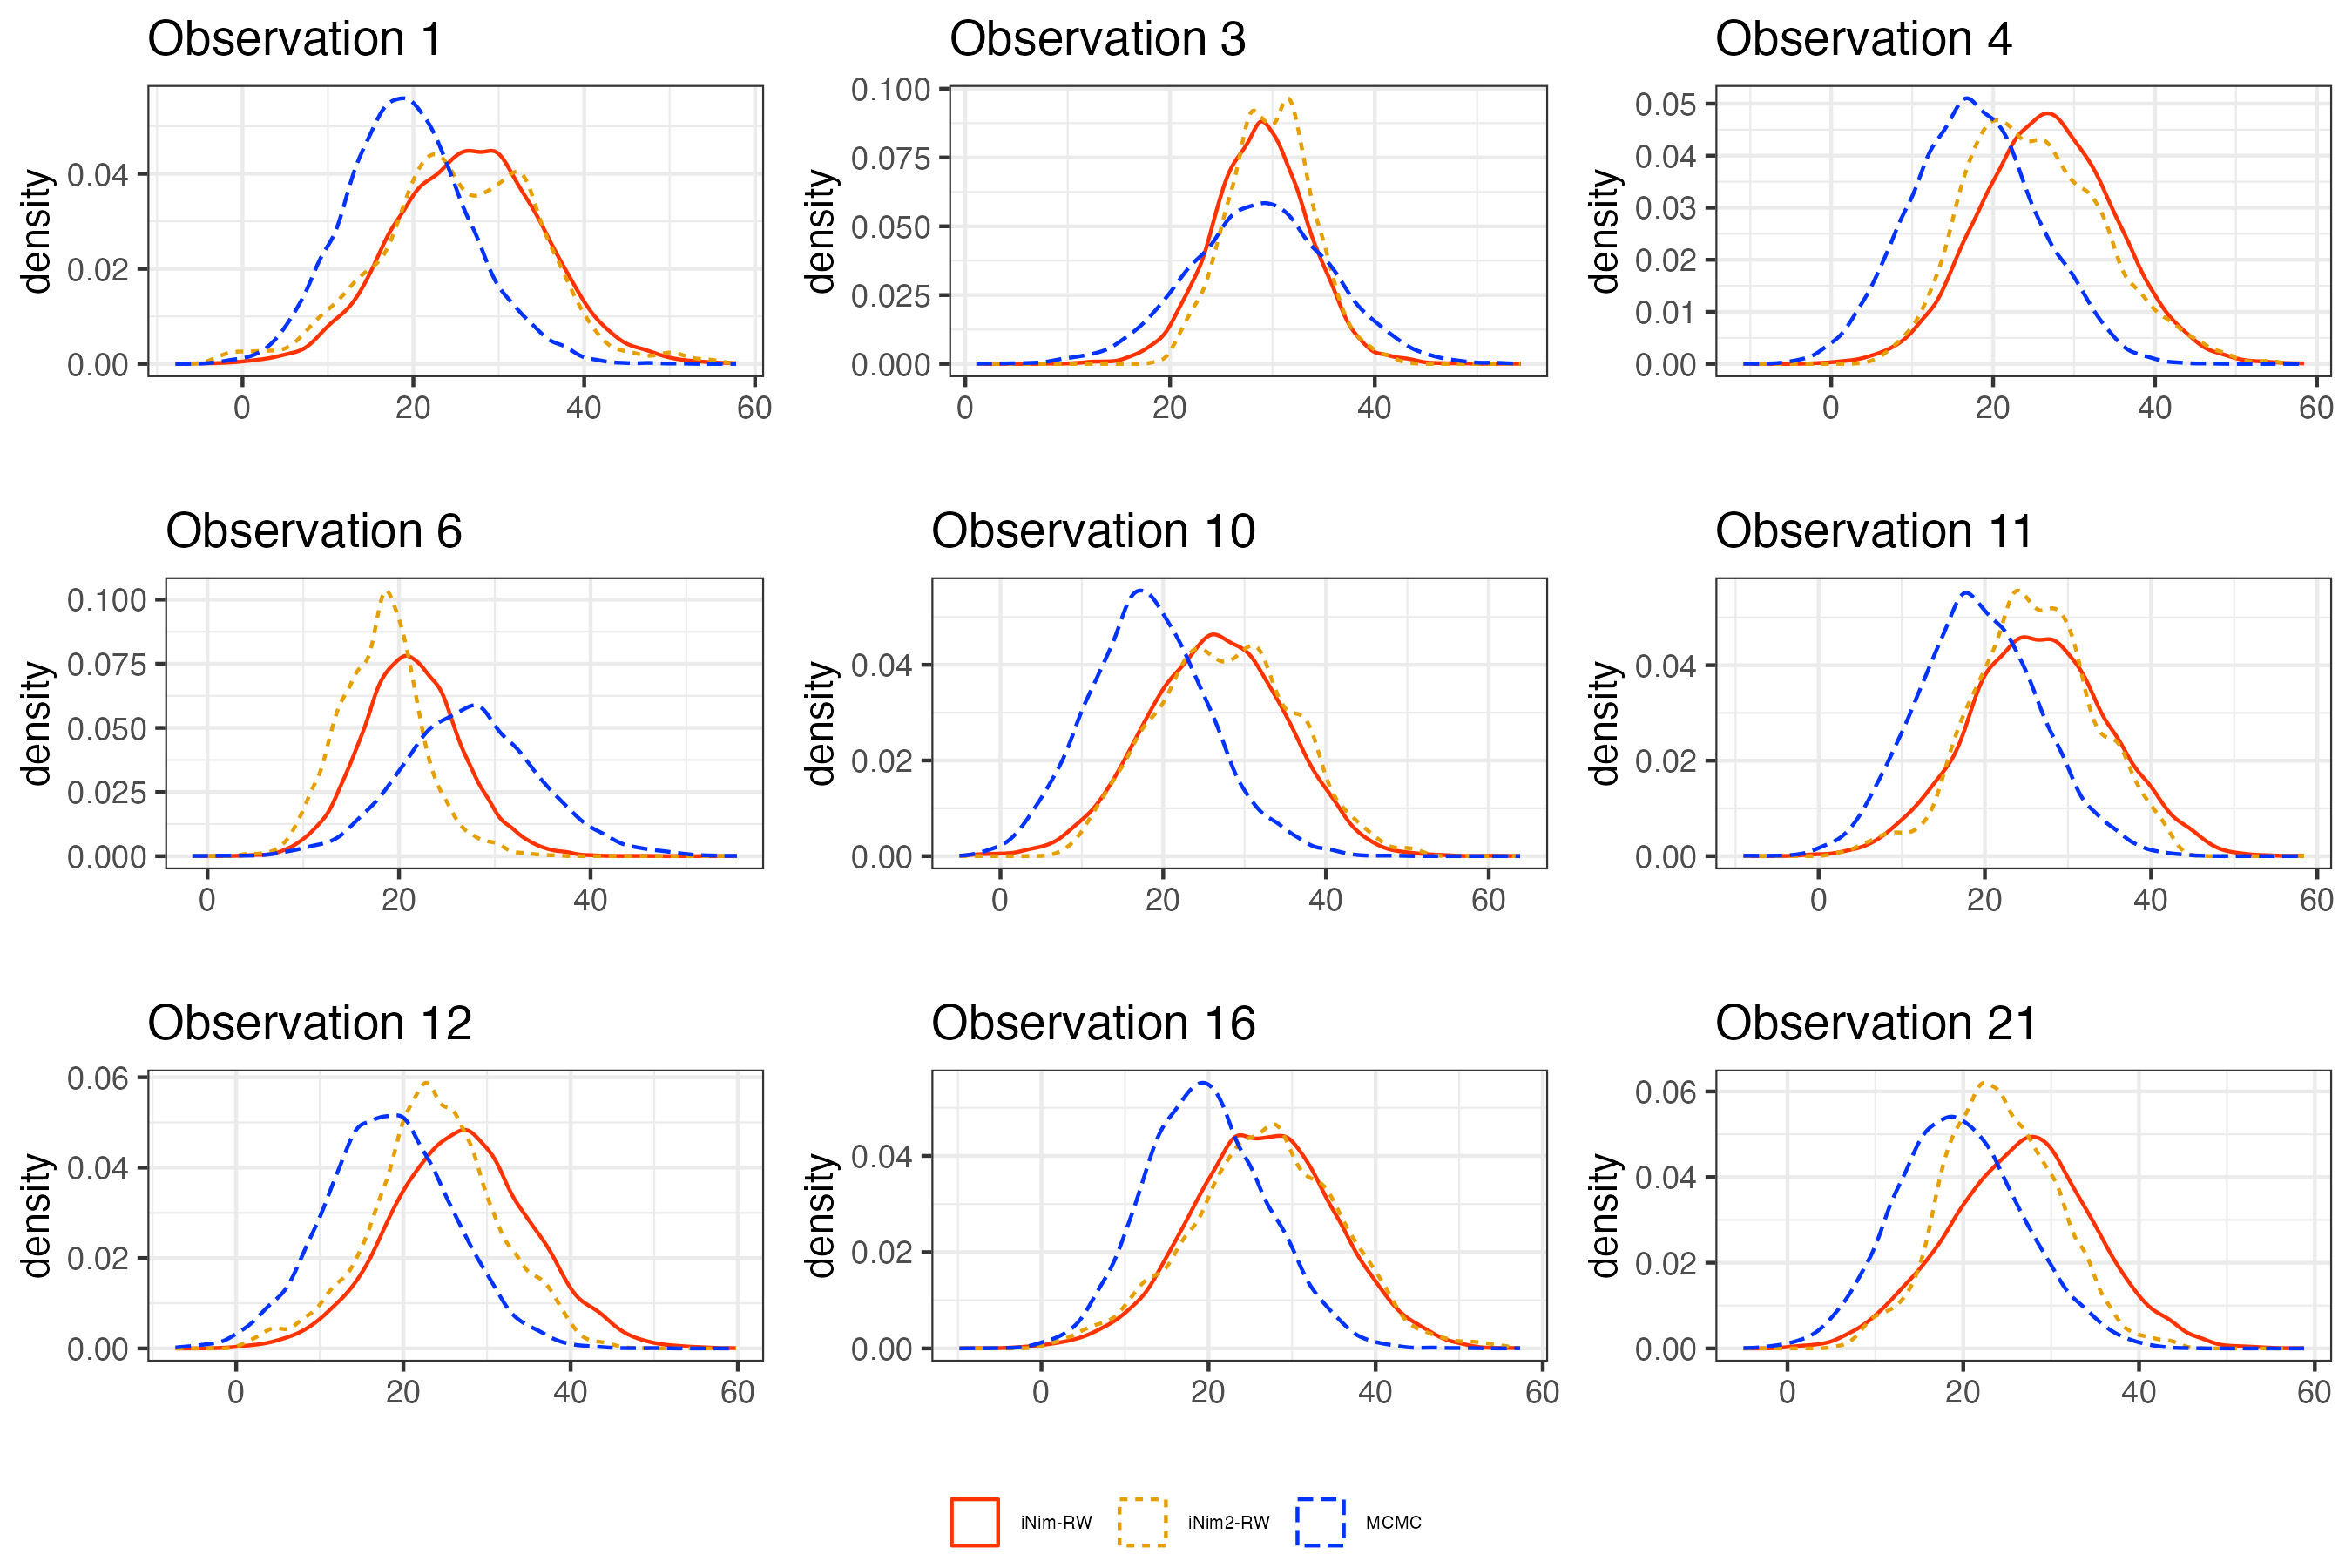
\includegraphics{results/missingRegression.png}

}

\caption{\label{fig-missingPlot}Posterior marginals of the imputed
values of the body mass index.}

\end{figure}

\hypertarget{tbl-missingCovs}{}
\begin{longtable}{llll}
\caption{\label{tbl-missingCovs}Summary of estimates of the parameters from the model with missing
covariates (with standard error in paranthesis). }\tabularnewline

\toprule
Parameter & iNim-RW & iNim-RW2 & MCMC\\
\midrule
\endfirsthead
\multicolumn{4}{@{}l}{\textit{(continued)}}\\
\toprule
Parameter & iNim-RW & iNim-RW2 & MCMC\\
\midrule
\endhead

\endfoot
\bottomrule
\endlastfoot
\cellcolor{gray!15}{$\alpha$} & \cellcolor{gray!15}{9.02 (6.1)} & \cellcolor{gray!15}{3.78 (23.9)} & \cellcolor{gray!15}{-0.21 (-0.21)}\\
$\beta_1$ & 34.13 (3.23) & 42.97 (11.13) & 14.16 (14.16)\\
\cellcolor{gray!15}{$\beta_2$} & \cellcolor{gray!15}{57.1 (9.91)} & \cellcolor{gray!15}{77.14 (15.3)} & \cellcolor{gray!15}{21.98 (21.98)}\\
$\beta_3$ & 6.03 (0.25) & 6.02 (0.85) & 5.58 (5.58)\\
\cellcolor{gray!15}{$\tau$} & \cellcolor{gray!15}{0 (0)} & \cellcolor{gray!15}{0 (0)} & \cellcolor{gray!15}{0 (0)}\\*
\end{longtable}

Figure \ref{fig-missingPlot} shows the posterior marginals of the
imputed missing body mass index values and Table \ref{tbl-missingCovs}
shows the summary of posterior distribution of the model parameters. The
posterior marginals obtained from the two INLA-MCMC approaches are
similar, but both are different from those estimated using MCMC. The
differences in the posterior marginals of the MCMC and INLA-MCMC
approaches could be due to the differences in the posterior predictive
distributions for missing values in the cholesterol from NIMBLe and
INLA. This consequently affects how the estimates of the model
parameters, which are different for all the three approaches (Table
\ref{tbl-missingCovs}).

\hypertarget{zero---inflated-poisson}{%
\subsubsection{Zero - inflated Poisson}\label{zero---inflated-poisson}}

We also used the proposed INLA-MCMC approaches to model count data with
excess zeroes using the zero-inflated Poisson regression model. The
zero-inflated Poisson model assigns a probability \(p\) that a count is
not zero, with this probability varying by a covariate.

Similar to the zero-inflated model in \citet{berild2022importance}, we
aim to predict the number of fishes caught by \(250\) groups of people
that went to a park based on the number of children (\(child\)) and
whether or not the group brought a camper into the park (\(camper\)) for
each group. The probability of getting counts greater than zero was
modeled as a logistic regression on the number of people (\(people\)).
The data used was accessed from the supplementary information in
\cite{berild2022importance}.

The model we aim to fit and the prior distribution of model parameters
are defined: \begin{equation}
\begin{split}
y_i | z_i &\sim ZIP(p_i, \mu_i), \quad i = 1, 2, \ldots, 250 \\
logit(p_i) &= \gamma_0 + \gamma_1 \text{people}_i \\
log(\mu_i) &= \beta_0 + \beta_1 \text{child}_i + \beta_2 \text{camper}_i \\
\text{Prior distributions:}\\
\gamma_0, \gamma_1 &\sim N(0, 0.0001) \\
\beta_0, \beta_1, \beta_2 &\sim N(0, 0.0001)\\
\end{split}
\end{equation} where \(\gamma_0\) and \(\gamma_1\) are the intercept and
covariate effect of \(people\) on the detection probability \(p\), and
\(\gamma_0\), \(\gamma_1\) and \(\gamma_2\) are the intercept, covariate
effect of number of children and whether the group brought a camper on
the mean counts of fishes. We chose
\(\mathbf{z}_{c} = (\gamma_0, \gamma_1)\) and
\(\mathbf{z}_{-c} = (\beta_0, \beta_1, \beta_2)\). New values of
\(\gamma_0\) and \(\gamma_1\) are proposed from normal distribution
centered around the mean estimates and the standard deviation equal to
three times the standard error estimates using the maximum likelihood
approach. The maximum likelihood estimates were obtained from
\textit{zeroinfl()} from the R-package \textbf{pscl} \citep{pscl}.

\hypertarget{tbl-zipSummary}{}
\begin{longtable}{lllll}
\caption{\label{tbl-zipSummary}Summary of estimates of the parameters from the zero-inflated Poisson
model (with standard error in paranthesis). The maximum likelihood
estimates (MLE) were obtained from fitting the model with the
\textbf{pscl} package. }\tabularnewline

\toprule
Parameter & MLE & iNim-RW & iNim2-RW & MCMC\\
\midrule
\endfirsthead
\multicolumn{5}{@{}l}{\textit{(continued)}}\\
\toprule
Parameter & MLE & iNim-RW & iNim2-RW & MCMC\\
\midrule
\endhead

\endfoot
\bottomrule
\endlastfoot
\cellcolor{gray!15}{$\beta_0$} & \cellcolor{gray!15}{1.6 (0.09)} & \cellcolor{gray!15}{0.76 (0.02)} & \cellcolor{gray!15}{0.77 (0.09)} & \cellcolor{gray!15}{0.21 (0.64)}\\
$\beta_1$ & -1.04 (0.1) & -1.03 (0.04) & -1.07 (0.07) & -1.05 (0.09)\\
\cellcolor{gray!15}{$\beta_2$} & \cellcolor{gray!15}{0.83 (0.09)} & \cellcolor{gray!15}{0.83 (0.01)} & \cellcolor{gray!15}{0.83 (0.05)} & \cellcolor{gray!15}{1.12 (0.34)}\\
$\gamma_0$ & 1.3 (0.37) & 1.11 (0.32) & 1.48 (0.25) & 1.29 (0.41)\\
\cellcolor{gray!15}{$\gamma_1$} & \cellcolor{gray!15}{-0.56 (0.16)} & \cellcolor{gray!15}{-0.49 (0.13)} & \cellcolor{gray!15}{-0.63 (0.11)} & \cellcolor{gray!15}{-0.6 (0.2)}\\*
\end{longtable}

The summary of the model parameters posterior distribution are presented
in Table \ref{tbl-zipSummary}. The estimates from the INLA-MCMC
approaches are similar to those estimated from MCMC and maximum
likelihood estimates.

\hypertarget{binomial-n-mixture-model-with-covariates-in-observation-process}{%
\subsubsection{Binomial N-Mixture model with covariates in observation
process}\label{binomial-n-mixture-model-with-covariates-in-observation-process}}

Modelling species abundance in space and time is a growing field in
applied ecology. Binomial N-Mixture model, a hierarchical model that
models latent abundance with a Poisson distribution and the observation
process given the latent abundance as a Binomial distribution, has been
widely used for such problems (\cite{kery2020applied, kery2017applied}
and references therein). \textbf{R-INLA} can be used fit the Binomial
N-mixture model, except for cases where there are observation level
covariates for the detection process
\citep{kery2020applied, meehan2017estimating}. In such instances, the
observation level covariates are aggregated and used in modelling the
detection process \citep{meehan2017estimating}.

We fit a Binomial N-Mixture model to mallard dataset that is publicly
available through the R-package \textbf{unmarked} \citep{unmarked}. The
dataset contains counts of mallard ducks (\textit{mallard.y}) collected
from \(239\) sites in Switzerland during two to three sampling occasions
in \(2002\). The dataset also contains abundance covariates called
\textit{mallard.site} which contains information on elevation
(\textit{elev}), forest cover (\textit{forest}), length of transect
(\textit{length}); and detection covariates called \textit{mallard.obs}
which contains information on survey date (\textit{data}) and survey
intensity (\textit{ivel}).

We are interested in predicting the total absolute abundance of mallard
ducks whilst accounting for imperfect detection. The model we aim to fit
and the prior distributions of the model parameters are as follows:
\begin{equation}
\begin{split}
y_{ij} &\sim Binomial(N_i, {p_{ij}}) \\
N_i & \sim Poisson(\lambda_i) \\
log(\lambda_i) &= \beta_0 + \beta_1 elev_i + \beta_2 length_i + \beta_3 forest_i \\
logit(p_{ij}) &= \alpha_{0} + \alpha_1 * ivel_{ij} + \alpha_2*data_{ij} +  \alpha_3*data_{ij}^{2} \\
\text{Prior distributions:}\\
\alpha_0, \alpha_1, \alpha_2, \alpha_3 &\sim N(0, 0.001) \\
\beta_0, \beta_1, \beta_2, \beta_3 &\sim N(0, 0.001)\\
\end{split}
\end{equation} where \(\beta_0\) is the intercept, \(\beta_1\) is the
effect of elevation, \(\beta_2\) is the effect of length of transect and
\(\beta_3\) is the effect of forest cover on the duck abundance;
\(\alpha_0\) is the intercept, \(\alpha_1\) is the effect of survey
intensity, \(\alpha_2\) and \(\alpha_3\) are the effect of linear and
quadratic effect of survey date respectively on the detection
probability.

Here, we split the latent states into two sets:
\(\mathbf{z}_{c} = (N_1, N_2, \ldots, N_{239}, \beta_0, \beta_1, \beta_2, \beta_3)\)
and \(\mathbf{z}_{-c} = (\alpha_0, \alpha_1, \alpha_2, \alpha_3)\). We
sample \(\mathbf{z}_{c}\) from MCMC by using the default slice sampler
for \(N_1, N_2, \ldots, N_{239}\) and the random walk block sampler for
\(\beta_0, \beta_1, \beta_2, \beta_3\); and \(\mathbf{z}_{-c}\) is
sampled from its posterior distribution from the conditional logistic
regression model fitted with \textbf{R-INLA}. The N-Mixture model was
also fitted with the R-package \textbf{unmarked} to obtain maximum
likelihood estimates for the parameters; and with MCMC using
\textbf{nimble} to obtain posterior distributions for the model
parameters.

\hypertarget{tbl-binNmix}{}
\begin{longtable}{llll}
\caption{\label{tbl-binNmix}Summary of estimates of the parameters from the Binomial N-Mixture model
(with standard error in paranthesis). The maximum likelihood estimates
(MLE) were obtained from the R-package \textbf{unmarked}. }\tabularnewline

\toprule
Parameter & MLE & iNim-RW & MCMC\\
\midrule
\endfirsthead
\multicolumn{4}{@{}l}{\textit{(continued)}}\\
\toprule
Parameter & MLE & iNim-RW & MCMC\\
\midrule
\endhead

\endfoot
\bottomrule
\endlastfoot
\cellcolor{gray!15}{$\alpha_0$} & \cellcolor{gray!15}{0.26 (0.22)} & \cellcolor{gray!15}{0.42 (0.06)} & \cellcolor{gray!15}{0.24 (0.22)}\\
$\alpha_1$ & 0.3 (0.18) & 0.23 (0.06) & 0.3 (0.17)\\
\cellcolor{gray!15}{$\alpha_2$} & \cellcolor{gray!15}{-0.37 (0.15)} & \cellcolor{gray!15}{-0.36 (0.02)} & \cellcolor{gray!15}{-0.33 (0.15)}\\
$\alpha_3$ & 0.01 (0.09) & 0.07 (0.01) & 0.04 (0.09)\\
\cellcolor{gray!15}{$\beta_0$} & \cellcolor{gray!15}{-1.99 (0.24)} & \cellcolor{gray!15}{-1.93 (0.29)} & \cellcolor{gray!15}{-1.91 (0.28)}\\
$\beta_1$ & -0.41 (0.13) & -0.5 (0.14) & -0.49 (0.14)\\
\cellcolor{gray!15}{$\beta_2$} & \cellcolor{gray!15}{-1.51 (0.25)} & \cellcolor{gray!15}{-1.36 (0.32)} & \cellcolor{gray!15}{-1.38 (0.31)}\\
$\beta_3$ & -0.71 (0.16) & -0.75 (0.18) & -0.76 (0.18)\\
\cellcolor{gray!15}{Ntotal} & \cellcolor{gray!15}{86 (NA)} & \cellcolor{gray!15}{80 (2.58)} & \cellcolor{gray!15}{83 (4.86)}\\*
\end{longtable}

The summary of the posterior distribution of model parameters are
presented in Table \ref{tbl-binNmix} and the posterior marginals of the
model parameters presented in Figure \ref{fig-binNmixPlot}. The results
are comparable across all the approaches.

\begin{figure}

{\centering 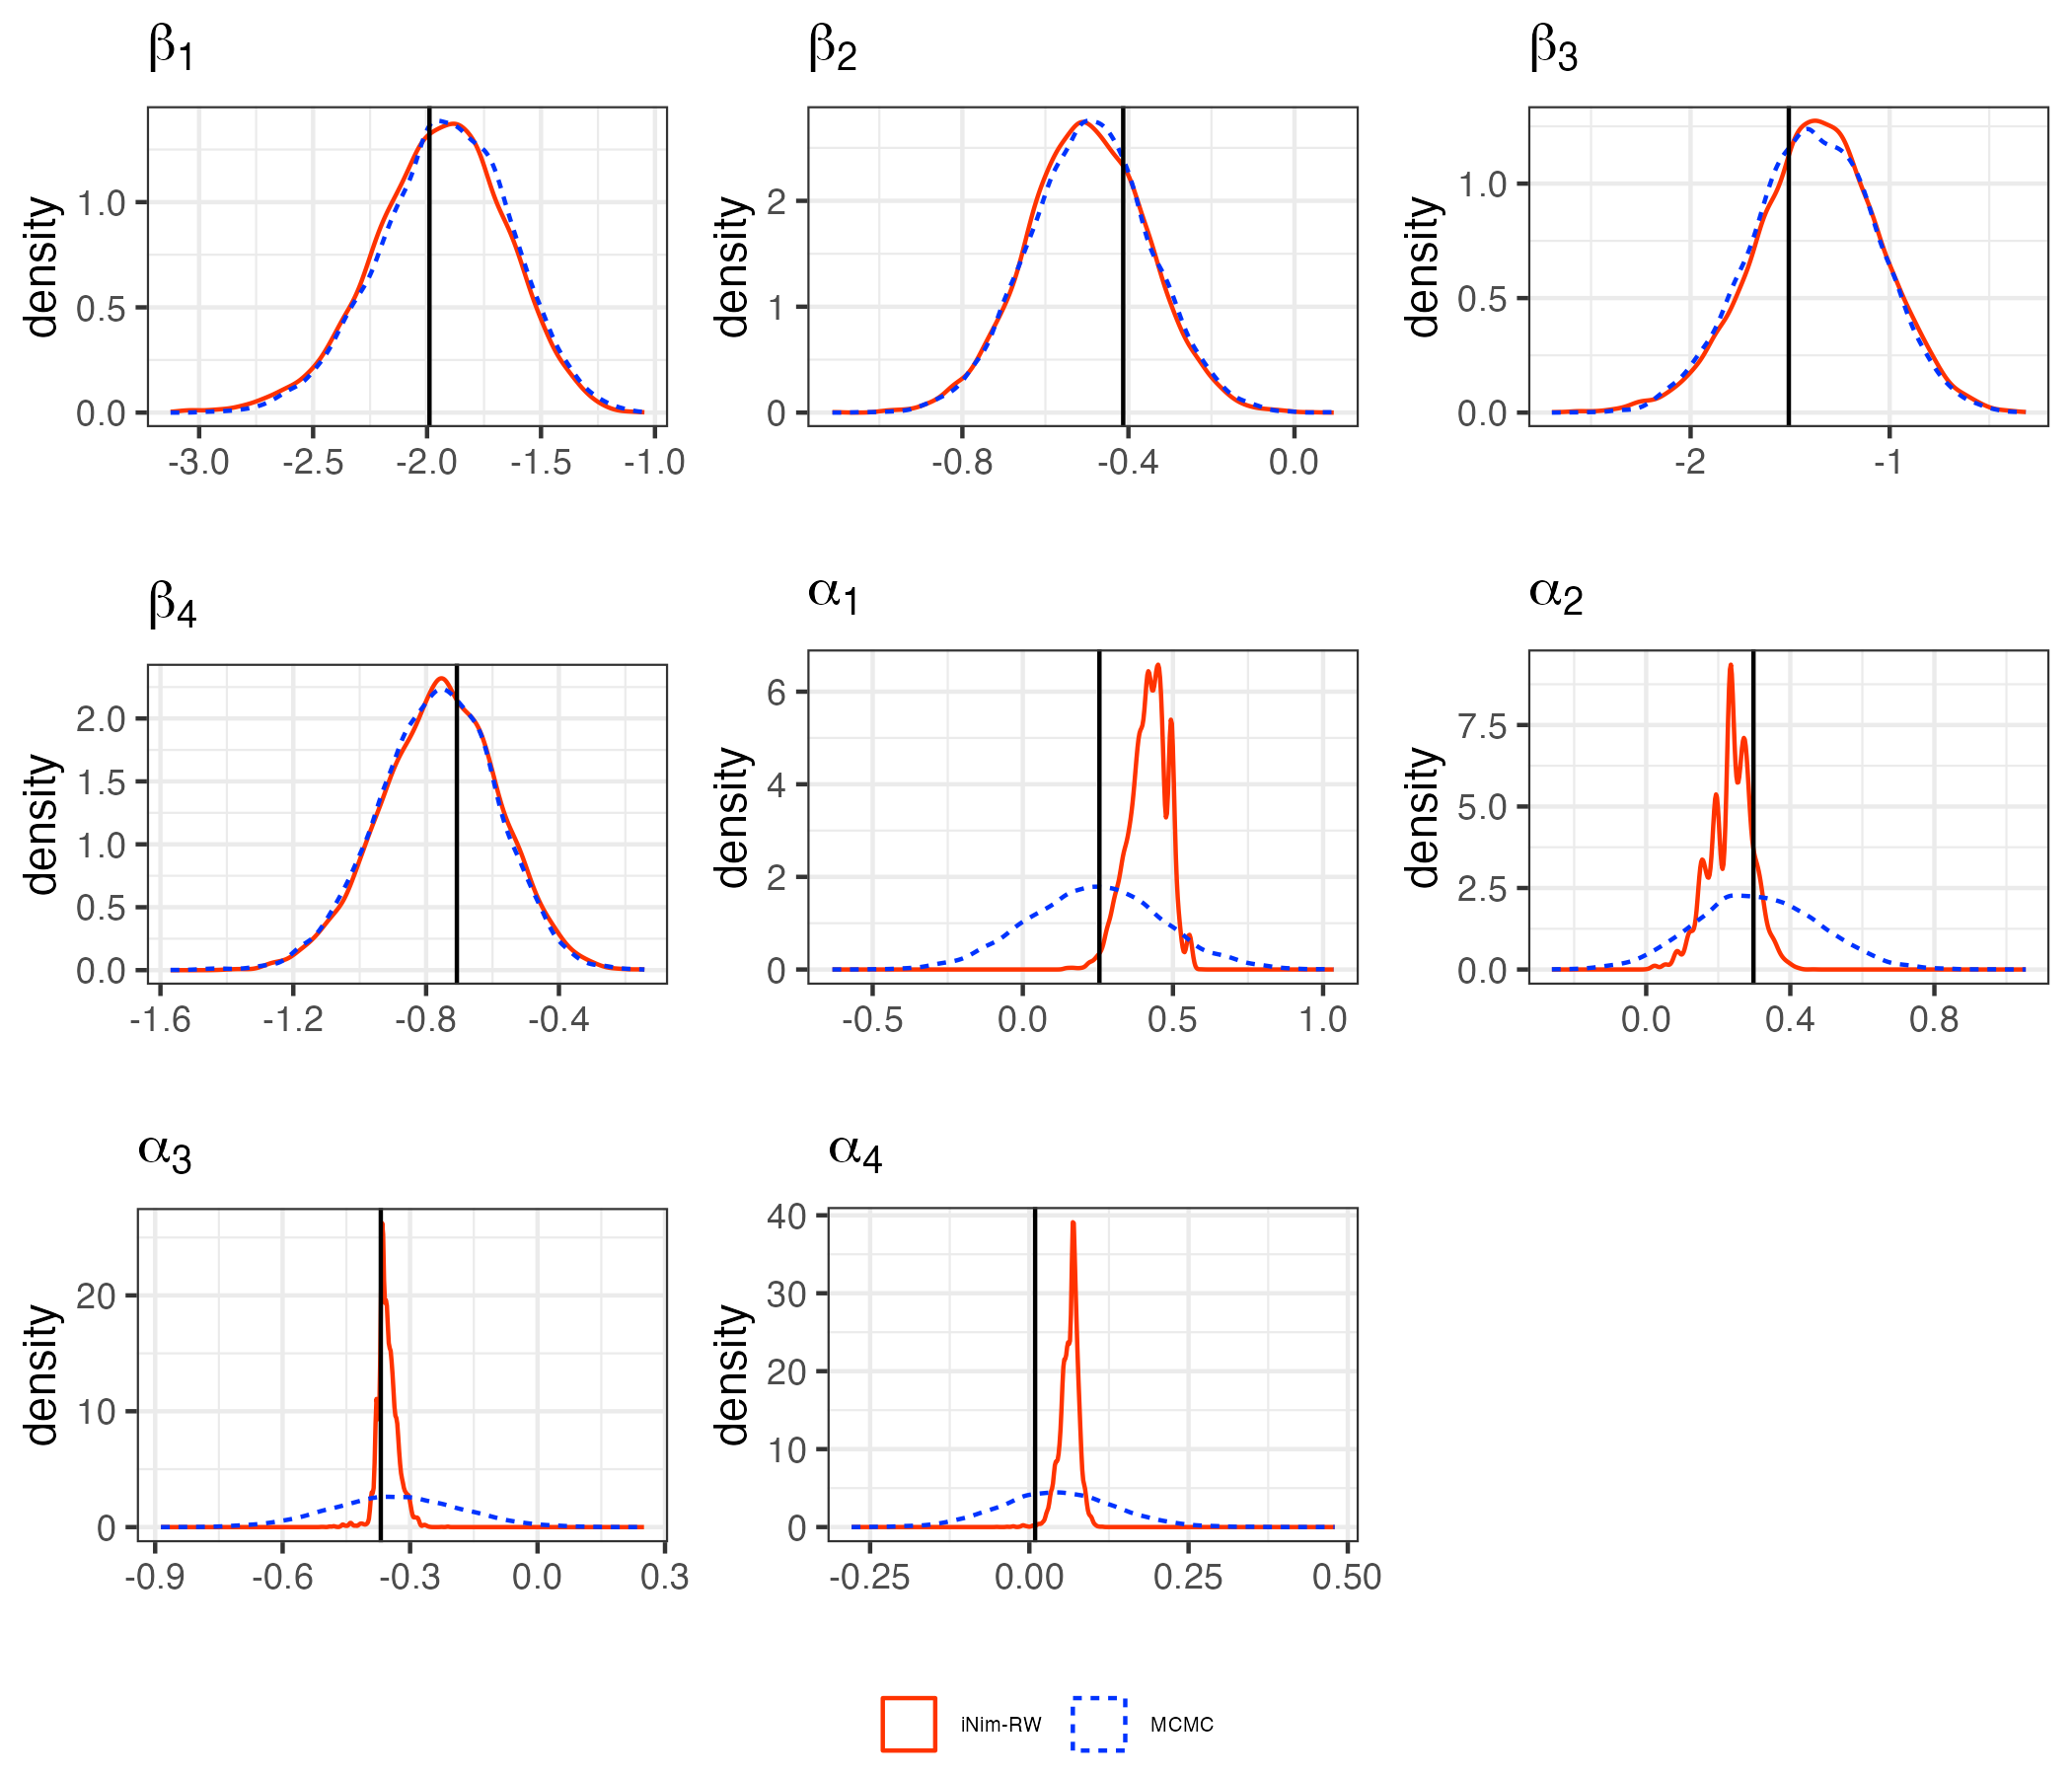
\includegraphics{results/binNmix.png}

}

\caption{\label{fig-binNmixPlot}Posterior marginals of the binomial
N-Mixture model parameters. The solid line indicates the maximum
likelihood estimate of the parameter using the \textbf{unmarked}
package.}

\end{figure}

\hypertarget{discussion}{%
\section{Discussion}\label{discussion}}

Using INLA-MCMC methodology for Bayesian inference is becoming an
integral part of applied statistics. By using this methodology, the
class of models fitted with \textbf{R-INLA} can be extended and the
computational time of fitting models with MCMC can also be reduced. This
methodology splits the model parameters into two mutually exclusive
sets: one set that will be sampled from MCMC and the other set that will
be sampled from the fitted conditional models using \textbf{R-INLA}.

Our study provided advancement in this methodology by showing how it can
be implemented with NIMBLE. Two alternative approaches of this
implementation are described in this study. The first approach is to use
\textbf{R-INLA} defined functions to write customized samplers and the
second approach is to use the \textbf{R-INLA} defined functions to write
a nimble distribution model to be used in NIMBLE's BUGS framework. Our
findings revealed that the marginal distribution of model parameters
from both approaches are comparable to those from MCMC, INLA and maximum
likelihood estimates.

Using NIMBLE for the INLA-MCMC methodology comes with its advantages.
Firstly, NIMBLE is very efficient in running MCMC as compared to other
competing software like JAGS and WinBUGS. NIMBLE also provides the
platform to integrate R-defined functions into the BUGS code, compile
them with C++ and efficiently generate samples using the numerous
sampling algorithms implemented in \textbf{nimble}.

Although implementing the INLA-MCMC methodology with NIMBLE has some
advantages, the longer computational times are inherited from the study
in \cite{gomez2018markov}. As noted in our introduction, fitting models
with \textbf{R-INLA} is very fast. However, integrating it with
\textbf{nimble}'s sampling algorithm - that generates samples
sequentially and makes calls to \textbf{R-INLA} for each iteration - can
substantially increase the computational time of the INLA-MCMC
methodology. This observation has already been noted in previous studies
by \cite{gomez2018markov} and \cite{berild2022importance}.

The number of calls made to \textbf{R-INLA} depends on the type of
sampling algorithm. For instance, if INLA-MCMC methodology is run for
\(M\) number of iterations, the random walk block sampling algorithm
calls \textbf{R-INLA} \(M\) times during the running of the MCMC step
(this ignores the number of calls made to \textbf{R-INLA} during the
model building and compilation steps in \textbf{nimble}). If we choose
the adaptive factor slice sampler \citep{tibbits2014automated} - which
we also tried to implement in this study - then NIMBLE will call the
\textbf{R-INLA} function for each of the univariate steps the sampling
algorithm makes along the eigen vector to update the posterior
distribution. If \(n_k\) steps are made at each of a multivariate
\(k\)-dimensional model parameter space during iteration
\(i \in \{1, 2, \ldots, M\}\), then the \textbf{R-INLA} call will be
made a total of \(n_k \times k \times M\) times.

Reducing the computational time can be achieved by using (adaptive)
importance sampling for MCMC, as done in \cite{berild2022importance}.
The concept of importance sampling has been implemented in the R-package
\textbf{nimbleSMC}, and further studies can explore integrating
\textbf{R-INLA} defined functions to fit models using the importance
sampling with INLA methodology. This reduction in computational time is
achieved due to the easy parallelization of the importance sampling
algorithm, which will simultaneously call \textbf{R-INLA} functions
multiple times at any given iteration. Moreover, the INLA framework can
be integrated into the NIMBLE platform, since the Laplace approximation
has been implemented in NIMBLE \citep{nimblemanual}. This would be
essential because the models that will be fitted can be compiled with
C++, which will increase the efficiency of our sampling algorithm.

The usage of NIMBLE for the INLA-MCMC approach plays to a wide range of
computational competency. Users who are new to the NIMBLE platform can
use the second alternative described in section \ref{alttwo}, where a
\textbf{R-INLA} function is embedded in the BUGS code as a NIMBLE
distribution function. The implemented samplers in \textbf{nimble} can
be used to easily obtain posterior distribution of model parameters
using the INLA-MCMC approach. However, there would be a limited control
on the \textbf{R-INLA} function calls, since NIMBLE would call this
function if the sampling of the model parameters depends on a random
variable defined in the \textbf{R-INLA} function. To have much control
of the number of calls, then the sampling algorithms have to be
customized (as described in section \ref{altone}). This approach comes
with having expertise in writing codes in the NIMBLE platform.

This study processes the \textbf{R-INLA} output at each iteration and
returns the marginal likelihood and samples from the posterior
distribution of the parameters in the fitted conditional models. We do
not save the output from \textbf{R-INLA} to perform any post-processing
Bayesian averaging of the fitted models, as done in
\cite{berild2022importance} and \cite{gomez2018markov}. Further work can
explore saving the \textbf{R-INLA} outputs as a NIMBLE list that can be
processed after the INLA-MCMC methodology have been successfully run
with \textbf{nimble}.

The proposed implementation presented in this study presents an
opportunity to integrate various computational methods on the same
platform. With the implementation of Laplace approximation in NIMBLE,
the INLA-MCMC method can be completely implemented in NIMBLE, without
external calls made to the \textbf{R-INLA}.

\hypertarget{code-availability}{%
\section{Code availability}\label{code-availability}}

All code and data used for this paper are on GitHub repository
\url{https://github.com/Peprah94/INLA_within_nimble}.

\hypertarget{conflict-of-interest}{%
\section{Conflict of interest}\label{conflict-of-interest}}

The authors declare no conflict of interest.

\hypertarget{author-contribution}{%
\section{Author contribution}\label{author-contribution}}

KPA led the writing of the manuscript and the implementation of the
methods. KPA and RBO were all involved in the idea conception.

\hypertarget{references}{%
\section*{References}\label{references}}
\addcontentsline{toc}{section}{References}

\renewcommand{\bibsection}{}
\bibliography{references.bib}




\end{document}
